\documentclass[twoside,twocolumn]{article}
\usepackage{amsfonts,amssymb,amsbsy,latexsym,amsmath,tabulary,graphicx,times,xcolor}

\usepackage{multirow}
\usepackage{amssymb}
\setcounter{tocdepth}{3}
\usepackage{graphicx}
\usepackage{makecell}
\usepackage{enumitem}
%\usepackage{todonotes}
\usepackage{multirow}   % Allows table elements to span several rows.
\usepackage{booktabs}   % Improves the typesettings of tables.
\usepackage{hyperref}  % Enables cross linking in the electronic document version. This package has to be included second to last.

\usepackage{booktabs}
\usepackage{arydshln}


\usepackage[nonindentfirst]{titlesec}
\usepackage{caption,abstract,fancyhdr}
\usepackage[utf8]{inputenc}
\usepackage[numbers,sort&compress]{natbib}
%\def\NormalBaseline{\def\baselinestretch{1.1}}
%\renewcommand{\bibnumfmt}[1]{\textbf{#1}.}

%\usepackage[overload]{textcase}

\def\oupIndent{1pt}

\usepackage[T1]{fontenc}
%\usepackage[paperheight=297mm,paperwidth=210mm,columnsep=1.93pc,right=17.5mm,left=20mm,top=20mm,bottom=20mm]{geometry}
%\usepackage[margin=1.5cm,columnsep=1.93pc,top=1in,bottom=2cm]{geometry}
\usepackage[paperheight=11.69in,paperwidth=8.27in,margin=1.5cm,headsep=.5cm,top=2cm,bottom=2.5cm,columnsep=12pt]{geometry}
\linespread{1.2} \date{}
\captionsetup[table]{labelfont={bf},labelsep=period}
\captionsetup[figure]{labelfont={bf},labelsep=period}
\def\abstractname{\fontsize{16pt}{19.2pt}\sffamily{Abstract}\selectfont}
\renewenvironment{onecolabstract} {\vspace*{-1pc}\trivlist\item[]\leftskip\oupIndent\par\vskip4pt\noindent\textit{{\abstractname}}\mbox{\null}\\ \textcolor[cmyk]{.77,.49,.38,.11}{\rule[.5pc]{\textwidth}{2pt}} \newline}{\par\noindent\endtrivlist}

\renewcommand{\bibnumfmt}[1]{#1.}


\makeatletter
\def\author#1{\gdef\@author{\hskip-\dimexpr(\tabcolsep)\hskip\oupIndent\parbox{\dimexpr\textwidth-\oupIndent}{#1}}}
\def\title#1{\gdef\@title{\raggedright\sffamily\bfseries\ifx\@articleType\@empty\else\@articleType\\\fi#1}}
\fancypagestyle{headings}{\renewcommand{\headrulewidth}{0pt}\renewcommand{\footrulewidth}{0pt}
\fancyhf{}\fancyhead[R]{{\rule{\textwidth}{.1pt}} \\ \RunningAuthor }\fancyhead[L]{{\rule{\textwidth}{0pt}} \\ \MakeUppercase{\journalTitle} }\fancyfoot[R]{\thepage}}\pagestyle{headings}
\fancypagestyle{plain}{\renewcommand{\headrulewidth}{0pt}\renewcommand{\footrulewidth}{0pt}\fancyhf{}\fancyhead[R]{{\rule{\textwidth}{.1pt}} \\ \RunningAuthor }\fancyhead[L]{{\rule{\textwidth}{0pt}} \\ \MakeUppercase{\journalTitle}}\fancyfoot[R]{\thepage}}
\let\@articleType\@empty \def\articletype#1{\gdef\@articleType{{\normalfont\underline{#1}}}}

\usepackage{titlesec}
\setcounter{secnumdepth}{5}
 \def\NormalBaseline{\def\baselinestretch{1.1}}
\titleformat{\section}[hang]{\NormalBaseline\filright\large\fontsize{16pt}{19.2pt}\itshape\sffamily}
{\large\thesection}
{}
{}
[{\color[cmyk]{.77,.49,.38,.11}\rule[3pc]{\columnwidth}{2pt}}]
\titleformat{\subsection}[hang]{\NormalBaseline\bfseries}
{}
{10pt}
{}
[]
\titleformat{\subsubsection}[hang]{\NormalBaseline\bfseries}
{}
{10pt}
{}
[]
\titleformat{\paragraph}[runin]{\NormalBaseline\bfseries}
{}
{10pt}
{}
[]
\titleformat{\subparagraph}[runin]{\NormalBaseline\filright\bfseries}
{}
{10pt}
{}
[]



\titlespacing{\section}{0pt}{1.5\baselineskip}{-2.5\baselineskip}
\titlespacing{\subsection}{0pt}{1.5\baselineskip}{.2\baselineskip}
\titlespacing{\subsubsection}{0pt}{1.5\baselineskip}{.2\baselineskip}
\titlespacing{\paragraph}{0pt}{.5\baselineskip}{10pt}
\titlespacing{\subparagraph}{0pt}{.5\baselineskip}{10pt}
\makeatother


%%%%%%%%%%%%%%%%%%%%%%%%%%%%%%%%%%%%%%%%%%%%%%%%%%%%%%%%%%%%%%%%%%%%%%%%%%
% Following additional macros are required to function some 
% functions which are not available in the class used.
%%%%%%%%%%%%%%%%%%%%%%%%%%%%%%%%%%%%%%%%%%%%%%%%%%%%%%%%%%%%%%%%%%%%%%%%%%
\usepackage{url,multirow,morefloats,floatflt,cancel,tfrupee}
\makeatletter
\AtBeginDocument{\@ifpackageloaded{textcomp}{}{\usepackage{textcomp}}}
\makeatother
\usepackage{colortbl}
\usepackage{xcolor}
\usepackage{pifont}
\usepackage[nointegrals]{wasysym}
\urlstyle{rm}
\makeatletter

\AtBeginDocument{
\expandafter\ifx\csname eqalign\endcsname\relax
\def\eqalign#1{\null\vcenter{\def\\{\cr}\openup\jot\m@th
  \ialign{\strut$\displaystyle{##}$\hfil&$\displaystyle{{}##}$\hfil
      \crcr#1\crcr}}\,}
\fi
}

\let\lt=<
\let\gt=>
\def\processVert{\ifmmode|\else\textbar\fi}
\let\processvert\processVert

\@ifundefined{subparagraph}{
\def\subparagraph{\@startsection{paragraph}{5}{2\parindent}{0ex plus 0.1ex minus 0.1ex}%
{0ex}{\normalfont\small\itshape}}%
}{}

% These are now gobbled, so won't appear in the PDF.
\newcommand\role[1]{\unskip}
\newcommand\aucollab[1]{\unskip}
  
\@ifundefined{tsGraphicsScaleX}{\gdef\tsGraphicsScaleX{1}}{}
\@ifundefined{tsGraphicsScaleY}{\gdef\tsGraphicsScaleY{.9}}{}
% To automatically resize figures to fit inside the text area
\def\checkGraphicsWidth{\ifdim\Gin@nat@width>\textwidth
	\tsGraphicsScaleX\textwidth\else\Gin@nat@width\fi}

\def\checkGraphicsHeight{\ifdim\Gin@nat@height>.9\textheight
	\tsGraphicsScaleY\textheight\else\Gin@nat@height\fi}

\def\fixFloatSize#1{\@ifundefined{processdelayedfloats}{\setbox0=\hbox{\includegraphics{#1}}\ifnum\wd0<\columnwidth\relax\renewenvironment{figure*}{\begin{figure}}{\end{figure}}\fi}{}}
\let\ts@includegraphics\includegraphics

\def\inlinegraphic[#1]#2{{\edef\@tempa{#1}\edef\baseline@shift{\ifx\@tempa\@empty0\else#1\fi}\edef\tempZ{\the\numexpr(\numexpr(\baseline@shift*\f@size/100))}\protect\raisebox{\tempZ pt}{\ts@includegraphics{#2}}}}

%\renewcommand{\includegraphics}[1]{\ts@includegraphics[width=\checkGraphicsWidth]{#1}}
\AtBeginDocument{\def\includegraphics{\@ifnextchar[{\ts@includegraphics}{\ts@includegraphics[width=\checkGraphicsWidth,height=\checkGraphicsHeight,keepaspectratio]}}}

\def\URL#1#2{\@ifundefined{href}{#2}{\href{#1}{#2}}}

%%For url break
\def\UrlOrds{\do\*\do\-\do\~\do\'\do\"\do\-}%
\g@addto@macro{\UrlBreaks}{\UrlOrds}
\makeatother
\def\floatpagefraction{0.8} 
\def\dblfloatpagefraction{0.8}
\def\style#1#2{#2}
\def\xxxguillemotleft{\fontencoding{T1}\selectfont\guillemotleft}
\def\xxxguillemotright{\fontencoding{T1}\selectfont\guillemotright}
%%%%%%%%%%%%%%%%%%%%%%%%%%%%%%%%%%%%%%%%%%%%%%%%%%%%%%%%%%%%%%%%%%%%%%%%%%

\newcommand{\mytodo}[1]{\textcolor{red}{#1}}
\newcommand{\todo}[1]{\textcolor{red}{#1}}

%{\hypersetup{colorlinks=false,linkcolor=green,urlcolor=red}}    

\newcommand{\emaillink}{
\hypersetup{%
  colorlinks=false,% hyperlinks will be black
  linkbordercolor=red,% hyperlink borders will be red
  pdfborderstyle={/S/U/W 0.5}% border style will be underline of width 1pt
}
}
\emaillink

\begin{document}

\title{A Study of Web Page Understandability\\ for Consumer Health Search}
\author{\textcolor{black}{\rule{\textwidth}{.1pt}}\vspace*{-.5pc} \textcolor{black}{\rule{\textwidth}{.1pt}} Joao Palotti\textsuperscript{1,3}, MSc;
            Guido Zuccon\textsuperscript{2}, PhD;
            Allan Hanbury\textsuperscript{3}, PhD\vspace*{-.5pc}\\\vspace*{-1pc}\textcolor{black}{\rule{\textwidth}{.1pt}}~\\[-3pt]\normalsize 
~\\\textsuperscript{1}{Qatar Computing Research Institute\unskip, Doha\unskip, Qatar} %, Email: jpalotti@hbku.edu.qa
~\\\textsuperscript{2}{Queensland University\unskip, Brisbane\unskip, Australia} %, Email: g.zuccon@qut.edu.au
~\\\textsuperscript{3}{Vienna University of Technology\unskip, Vienna\unskip, Austria} %, Email: hanbury@ifs.tuwien.ac.at}
%
\\
%
\\
%
\textbf{Corresponding Author:}\\
Joao Palotti, MSc.\\
Hamad Bin Khalifa University\\
Qatar Computing Research Institute\\
Education City\\
Doha\\
Qatar\\
Email: \href{mailto:jpalotti@hbku.edu.qa}{jpalotti@hbku.edu.qa}
}

\def\RunningAuthor{Palotti, Zuccon and Hanbury}\def\journalTitle{Journal of Medical Internet Research}

\twocolumn[ \maketitle {\begin{onecolabstract}
\textbf{Background:} Understandability plays a key role in ensuring that people accessing health information are capable of gaining insights that can assist them with their health concerns and choices. The access to unclear or misleading information has been shown to negatively impact on the health decisions of the general public.

\textbf{Objective:} We investigated methods to estimate the understandability of health Web pages and used these to improve the retrieval of information for people seeking health advice on the Web

\textbf{Methods:} Our investigation considered methods to automatically estimate the understandability of health information in Web pages, and it provided a thorough evaluation of these methods using human assessments as well as an analysis of pre-processing factors affecting understandability estimations, and associated pitfalls. Furthermore, lessons learnt for estimating Web page understandability were applied to the construction of retrieval methods with specific attention to retrieving information understandable by the general public.

\textbf{Results:} We found that machine learning techniques were more suitable to estimate health Web page understandability than traditional readability formulas, which are often used as guidelines and benchmarking by health information providers on the Web. Learning to rank effectively exploited these estimates to provide the general public with more understandable search results.

\textbf{Conclusions:} The findings reported in this article are important for specialised search services tailored to support the general public in seeking health advice on the Web, as they document and empirically validate state-of-the-art techniques and settings for this domain application.

%\textit{OLD ABSTRACT: In this paper, we investigated methods to estimate the understandability of health Web pages and used these to improve the retrieval of information for people seeking health advice on the Web.  Understandability plays a key role in ensuring that people accessing health information are capable of gaining insights that can assist them with their health concerns and choices. The access to unclear or misleading information has been shown to negatively impact on the health decisions of the general public. Our investigation considered methods to automatically estimate the understandability of health information in Web pages, and it provided a thorough evaluation of these methods using human assessments as well as an analysis of pre-processing factors affecting understandability estimations, and associated pitfalls. Furthermore, lessons learnt for estimating Web page understandability were applied to the construction of retrieval methods with specific attention to retrieving information understandable by the general public. We found that machine learning techniques were more suitable to estimate health Web page understandability than traditional readability formulas, which are often used as guidelines and benchmarking by health information providers on the Web. Learning to rank effectively exploited these estimates to provide the general public with more understandable search results. These results are important for specialised search services tailored to support the general public in seeking health advice on the Web.}

\textcolor{black}{\rule{\textwidth}{.2pt}} \\ \smallskip\noindent\textbf{KEYWORDS: }{Consumer Health Search; Document Understandability; Document Readability\newline}
\end{onecolabstract}}]\saythanks 



\section{Evaluation Metrics of Understandability in Search Engines}
\label{chp:evaluation_metrics}

One of the first notions of relevance was straightforward: a document is relevant to a query if the topic of the information retrieved matches the topic of the request.
This was called \textit{topical relevance} by Eisenberg and Schamber~\cite{eisenberg88} and measured whether a document was ``on the topic'' or ``on the subject''.
Due to its simplicity and clear definition~\cite{borlund03}, this notion was adopted by most of the modern evaluation tasks, such as TREC\footnote{\url{http://trec.nist.gov}}, CLEF\footnote{\url{http://www.clef-initiative.eu/}} and NTCIR\footnote{\url{http://http://research.nii.ac.jp/ntcir/index-en.html}}, which heavily rely on evaluation metrics that exclusively measure the topical relevance of documents~\cite{voorhees05}.
Recently extensions were made based on notions of novelty and diversity (e.g.,~\cite{clarke09}), but these new metrics still mainly consider relevance with respect to document topicality.

However, document relevance cannot be attributed to just one factor such as topicality, instead it is multidimensional and situational~\cite{borlund03}.
Early research~\cite{saracevic75,swanson86,harter92}, reviewed by Borlund divided relevance into two classes: (1) objective or system-based relevance and (2) subjective or human based relevance~\cite{borlund03}. 
This first class of relevance exclusively refers to the document ``aboutness'' aforementioned and it is context-free, while the second one refers to the subjective factors in both user and documents and it is context dependent.
A large body of subsequent research was dedicated to identifying the subjective aspects of relevance.
Park, for example, identified individual's subject knowledge, professional training, and educational background as a user-based influential factor, while scarcity, availability, timeliness, and scope as document-based factors~\cite{park93}.
Schamber published a compiling and non-exhaustive list of 80 relevance criteria suggested in the literature~\cite{schamber94}.
%
In the consumer health search domain, William Hersh highlighted two important factors to be considered by modern search engines~\cite{hersh08}: understandability and information trustworthiness. 
This paper focus on the community efforts to integrate these two dimensions in the evaluation of consumer health search systems.
%This thesis focus on the first one.

Early efforts to integrate understandability into information retrieval evaluation was made by Zuccon and Koopman~\cite{zuccon14} and enhanced later by Zuccon~\cite{zuccon16}.
Metrics such as $uRBP$ and $uRBPgr$, built upon the Rank Biased Precision metric (RBP)~\cite{moffat08}, were widely used in recent evaluation campaigns in the context of CLEF eHealth to combine understandability of documents with topical relevance.
$uRBP$, short for understandability-biased RBP and its graded version, $uRBPgr$, merge the relevance and understandability scores of a document into a unique score following the gain-discount framework by Carterette~\cite{carterette11}.

While Zuccon's framework can be successfully used to compare results across systems, as intended by evaluation campaigns such as CLEF eHealth, it is not trivial to identify how the retrieval performance of different dimensions affect the final score outputted by this framework.
We shall see in this paper that the early combination of scores make it difficult to interpret whether improvements (deterioration) are due to more (less) understandable or more (less) topical documents being retrieved.

What We propose is an alternative metric $H$ which uses a harmonic mean function to combine scores earlier calculated for each dimension.
In order to fairly compare our framework with Zuccon's, we also modify the RBP metric in our framework, resulting in the $H_{RBP}$ metric.

We shall review Zuccon's framework in Section~\ref{sec:understandability_metrics}. 
Our proposed alternative framework is presented in Section~\ref{sec:extension}.
We compare both frameworks through simulations in Section~\ref{sec:simulations}.
Finally, a summary is done in Section~\ref{sec:eval_summary}.

%%%%%%%%%%%%%%%%%%%%%%%%%%%%%%%%%%%%%%%%%%%%%%%%%%%%%%%%%%%%%%%%%%%%%%%%%%%%%%%%%%%%%%%%%%%%%%%%%%%%%%%%%%%%%%%%%%%%%%%%%%%%%%%%
%%%%%%%%%%%%%%%%%%%%%%%%%%%%%%%%%%%%%%%%%%%%%%%%%%%%%%%%%%%%%%%%%%%%%%%%%%%%%%%%%%%%%%%%%%%%%%%%%%%%%%%%%%%%%%%%%%%%%%%%%%%%%%%%
%%%%%%%%%%%%%%%%%%%%%%%%%%%%%%%%%%%%%%%%%%%%%%%%%%%%%%%%%%%%%%%%%%%%%%%%%%%%%%%%%%%%%%%%%%%%%%%%%%%%%%%%%%%%%%%%%%%%%%%%%%%%%%%%
%%%%%%%%%%%%%%%%%%%%%%%%%%%%%%%%%%%%%%%%%%%%%%%%%%%%%%%%%%%%%%%%%%%%%%%%%%%%%%%%%%%%%%%%%%%%%%%%%%%%%%%%%%%%%%%%%%%%%%%%%%%%%%%%




\section*{Related Work}
%\section{Related Work}

\label{sec:related}
Understandability refers to the ease of comprehension of the information presented to a user. Put in other words, health information is understandable ``when consumers of diverse backgrounds and varying levels of health literacy can process and explain key messages''~\cite{shoemaker2014development}. Often the terms understandability and readability are used interchangeably: we use readability to refer to formulas that estimate how easy is to understand a text, usually based on its words and sentences. We use understandability to refer to the broader concept of ease of understanding: this is affected by text readability (as increasing readability tends to improve understanding), but may also be influenced by how legible a text is and its layout, including e.g., the use of images to explain difficult concepts.

There is a large body of literature that has examined the understandability of Web health content when the information seeker is a member of the general public. For example, Becker reported that the majority of health Web sites are not well designed for the elderly~\cite{becker04}, while Stossel et al. found that  health education material on the Web is not written at an adequate reading level~\cite{stossel12}.
A common finding of these studies is that, in general, health content available on Web pages is often hard to understand by the general public; this includes content that is retrieved in top ranked positions by current commercial search engines~\cite{graber99,fitzsimmons10,wiener13,patel13,atcherson14,meillier17}.

Previous Linguistics and Information Retrieval (IR) research has attempted to devise computational methods for the automatic estimation of text readability and understandability, and for the inclusion of these within search methods or their evaluation. Computational approaches to understandability estimations include (1) \textit{readability formulas}, which generally exploit word surface characteristics of the text, (2) \textit{machine learning} approaches, (3) matching with specialised \textit{dictionaries or terminologies}, often compiled with information about understandability difficulty.

Measures such as Coleman-Liau Index (CLI))~\cite{cli75}, Dale-Chall Index (DCI)~\cite{dale48} and Flesch Reading Easy (FRE)~\cite{flesch75}
%, Simple Measure of Gobbledygook~\cite{smog69} 
belong to the first category. These measures generally rely on surface-level characteristics of text, such as characters, syllables and word counts~\cite{dubay04}. While these measures have been widely used in studies investigating the understandability of health content retrieved by search engines (e.g.,~\cite{becker04,graber99,fitzsimmons10,stossel12,wiener13,patel13,atcherson14,meillier17}), Palotti et al. found that they are heavily affected by the methods used to extract text from the HTML source~\cite{palotti15}. They were able to identify specific settings of an HTML preprocessing pipeline that provided consistent estimates. We shall revisit this work in more details in Section~\ref{sec:which_preprocessing}, as we further investigate this problem by comparing the effect of HTML preprocessing on text understandability estimations in light of explicit human assessments. 

The use of machine learning to estimate understandability forms an alternative approach. Earlier research explored the use of statistical natural language processing and language modelling~\cite{liu04,collins05,heilman07} as well as linguistic factors, such as syntactic features or lexical cohesion~\cite{pitler08}. While we replicated here many of the features devised in these works, they focus on estimating readability of general English documents rather than medical ones. In the medical domain, Zeng et al. explored features such as word frequency in different medical corpora to estimate concept familiarity, which prompted the construction of the Consumer Health Vocabulary (CHV)~\cite{zeng05,zeng06,zeng08}.  

The actual use of CHV or other terminologies such as the Medical Subject Headings (MeSH) belongs to the third category of approaches. The CHV is a prominent medical vocabulary dedicated to mapping layperson vocabulary to technical terms~\cite{zeng06}. It attributes a score for each of its concepts with respect to their difficulty, with lower/higher scores for harder/easier concepts. Researchers have evaluated CHV in tasks such as document analysis~\cite{leroy08} and medical expertise prediction~\cite{palotti14}.
The hierarchy of MeSH was previously used in the literature to identify hard concepts, assuming that a concept deep in the hierarchy is harder than a shallow one~\cite{yan11}. Other approaches combined vocabularies with word surface characteristics and syntactic features, like part of speech, into a unique readability measure~\cite{kim2007beyond}.

In this work, we investigated approaches to estimate understandability from each of these categories. We further extended Palotti et al.'s work to understand the influence of HTML preprocessing on automatic understandability methods and establish best practices. 

Some prior work has attempted to use understandability estimations for improving search results in consumer health search; as well as methods to evaluate retrieval systems that do account for understandability along with topical relevance. Palotti et al.~\cite{palotti2016ranking} have used learning to rank with standard retrieval features along with features based on readability formulas and medical lexical aspects to determine understandability. Van Doorn et al.~\cite{van2016balancing} have shown that learning a set of rankers that provide trade-offs across a number of relevance criteria, including readability/understandability, increases overall system effectiveness.   
Zuccon and Koopman~\cite{zuccon14}, and later Zuccon~\cite{zuccon2016understandability}, have proposed and investigated a family of measures based on the gain-discount framework, where the gain of a document is influenced by both its topical relevance and its understandability. They showed that, although generally correlated, topical-relevance evaluation alone provides differing system rankings compared to understandability-biased evaluation measures. 
In this work we further explored the development of retrieval methods that combine signals about topical relevance and understandability. 



\section{Data and Resources}
\label{sec:data}

\subsection{Data Collections}

In this paper we investigate methods to estimate Web page understandability, including the effect HTML preprocessing pipelines and heuristics have, and their search effectiveness when employed within retrieval methods. To obtain both topical relevance\footnote{We refer to this simply as relevance in the reminder of the paper, when this does not cause confusion.} and  understandability assessments, we used the data from the CLEF 2015 and 2016 eHealth collections. 

The CLEF 2015 collection contains 50 queries and 1,437 documents that have been assessed relevant by clinical experts and have an assessment for understandability~\cite{clef15}. Documents in this collection are a selected crawl of health websites, of which the majority are certified HON websites.
The CLEF 2016 collection contains 300 queries and 3,298 relevant documents that also have been assessed with respect to understandability~\cite{clef16}. Documents in this collection belong to the ClueWeb12 B13 corpus, and thus are general English Web pages, not necessarily targeted to health topics, nor of a controlled quality (as are instead HON certified pages). 
Understandability assessments were provided on a 5-point Likert scale for CLEF 2015, and on a $[0,100]$ range for CLEF 2016 (0 indicates highest understandability). 

To support the investigation in Section~\ref{sec:which_preprocessing} (evaluation of preprocessing pipelines and heuristics), we further considered correlations between multiple human assessors (inter-assessor agreement). For CLEF 2015, we used the publicly available additional assessments made by unpaid medical students and health consumers collected by Palotti et al.~\cite{palotti16b} in a study of how medical expertise affects assessments. For CLEF 2016 we  collected understandability assessments for 100 documents. Three members of our research team, which did not author this paper, were recruited to provide the assessments. The Relevation tool~\cite{koopman14} was used to assist with the assessments, mimicking the settings used in CLEF.

In the experiments, we used Pearson, Kendall and Spearman correlations to compare the understandability assessments of human assessors with estimations obtained by the considered approaches, under all combinations of pipelines and heuristics. Pearson correlation is used to calculate the strength of the linear relation between two variables, while Kendall and Spearman measure the rank correlations between the variables. We opted to report all three correlation coefficients to allow for a thorough comparison to other work, as they are equally used in the literature. 

\subsection{Evaluation Measures}

For the retrieval experiments in Section~\ref{sec:results}, we use evaluation measures that use both relevance and understandability. The uRBP measure~\cite{zuccon2016understandability} extends rank biased precision (RBP) to scenarios where multiple relevance dimensions are used. Formally, the measure is formulated as $uRBP(\rho) = (1 - \rho) \sum_{k=1}^{K} \rho^{k-1} r(d@k) u(d@k)$, where $r(d@k)$ is the gain for retrieving a relevant document at rank $k$ and $u(d@k)$ is the gain for retrieving a document of a certain understandability at rank $k$; $\rho$ is the RBP persistence parameter. This measure was an official metric used in CLEF (we also set $\rho=0.8$). 

A drawback of uRBP is that relevance and understandability are combined into a unique evaluation score, thus making it difficult to interpret whether improvements are due to more understandable or more topical documents being retrieved. To overcome this, we first separately calculate an RBP value for relevance and another for understandability, and then combine them into a unique effectiveness measure:

\begin{itemize}[leftmargin=*]
	\item $RBP_r@n(\rho)$: uses the relevance assessments for the top $n$ search results (i.e. this is the common RBP). In this paper, we regarded a document as topically relevant if assessed as somewhat relevant or highly relevant.
	
    \item $RBP_u@n(\rho)$: uses the understandability assessments for the top $n$ search results. In this paper, we regarded a document as understandable (1) for CLEF 2015 if assessed easy or somewhat easy to understand; (2) for CLEF 2016 if its assessed understandability score was smaller than a threshold $U$ (we used $U = 40$ \footnote{This choice for $U$ is based on the distribution of understandability assessments. This distribution can be found in the online appendix.}).
	
    \item $HRBP@n(\rho) = 2 \times \frac{RBP_r@n \times RBP_u@n}{RBP_r@n + RBP_u@n}$: combines the previous two RBP values into a unique measurement using the harmonic mean (in the same fashion that the $F_1$ measure combines recall and precision).
\end{itemize}

\noindent For all measures we set $n=10$ because shallow pools were used in CLEF along with measures that focused on the top 10 search results (including $RBP_r@10$).

Along with these measures of search effectiveness, we also reported the number of unassessed documents, the RBP residual, and  $RBP_r@10^*$, $RBP_u@10^*$ and $HRBP^*$, i.e. the corresponding measures calculated by ignoring unassessed documents. We did this to minimise pool bias since the pools built in CLEF were of limited size, and the investigated methods retrieved a substantial number of unassessed documents.


\subsection{Preprocessing Pipelines and Heuristics}
\label{sec:pipelines}

We study the influence the preprocessing of Web pages have on the estimation of understandability when using the evaluated methods present in Section~\ref{sec:proxies}. We do so by comparing the combination of a number of preprocessing pipelines, heuristics, and understandability estimation methods with human assessments of Web page understandability. 
Our experiments extend those by Palotti et al.~\cite{palotti15}, who only evaluated surface level readability formulas and did not compare their results against human assessments. 

To extract the content of a Web page from the HTML source we test: BeautifulSoup~\cite{bs4} (\textit{Naive}), which just naively removes HTML tags, Boilerpipe~\cite{kohlschutter10} (\textit{Boi}) and Justext~\cite{jan11} ({Jst}), which eliminates boilerplate text together with HTML tags. 
%Palotti et al.'s data analysis highlighted that the text in HTML tags often missed a correct punctuation mark and thus the text extracted from HTML fields like titles, menus, tables and lists could be interpreted as many short sentences or few very long sentences, depending on whether a period was forced at the end of fields/sentences. We thus implement the same two heuristics devised by them to deal with this: \textit{ForcePeriod (FP)} and \textit{DoNotForcePeriod (DNFP)}. The FP heuristic forces a period at the end of each extracted HTML field; while the DNFP does not. 
Palotti et al.'s data analysis highlighted that the text in HTML fields like titles, menus, tables and lists often missed a correct punctuation mark and thus the text extracted from them
could be interpreted as many short sentences or few very long sentences, depending on whether a period was forced at the end of fields/sentences. We thus implement the same two heuristics devised by Palotti et al. to deal with this: \textit{ForcePeriod (FP)} and \textit{DoNotForcePeriod (DNFP)}. The FP heuristic forces a period at the end of each extracted HTML field, while the DNFP does not. 


\subsection{Additional Resources}

Because of space limitations, in this paper we only report a subset of the results; the remaining results (which show similar trends to those reported here) are made available in an online appendix for completeness: {\url{https://sites.google.com/view/www2018-sub341}. All data and code will be shared on GitHub upon acceptance. 

%\begin{figure*}[th!]
%   \centering
%   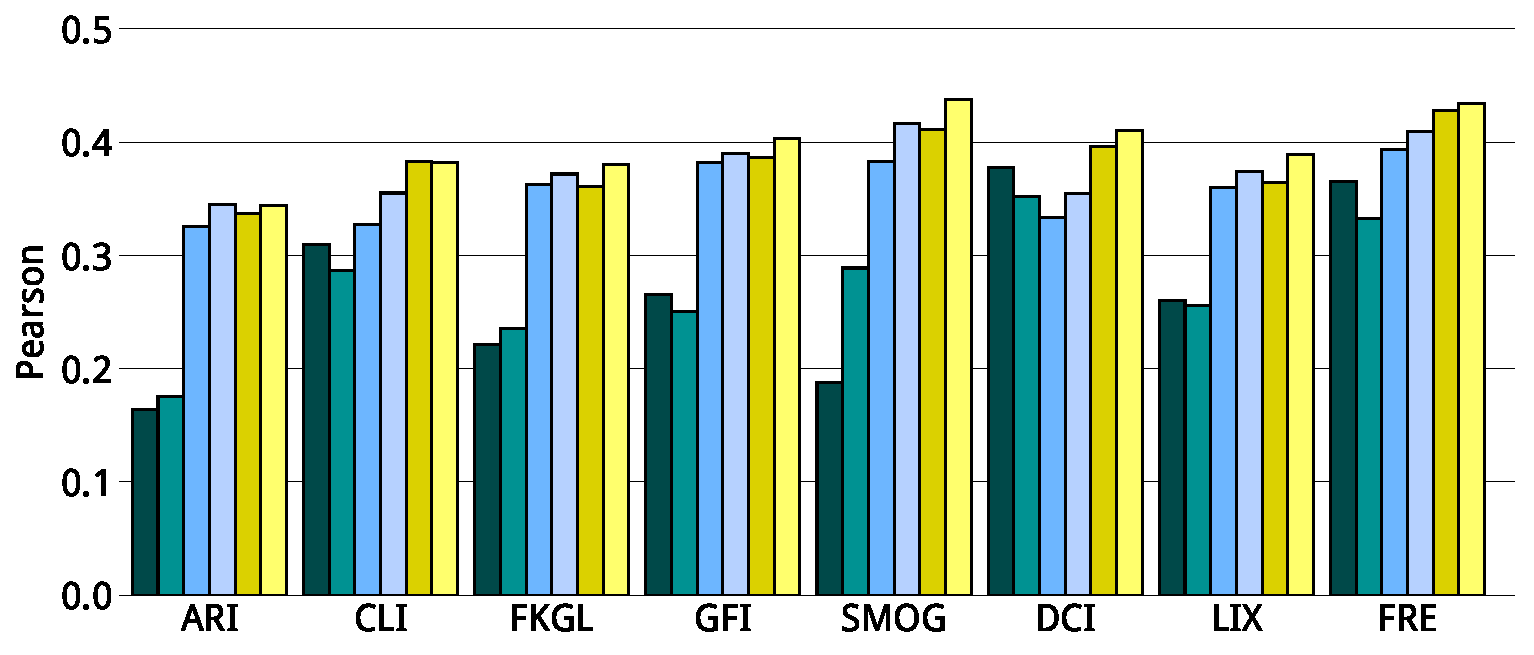
\includegraphics[width=.45\textwidth]{graphics/bar_corr_pearson15_values}
%   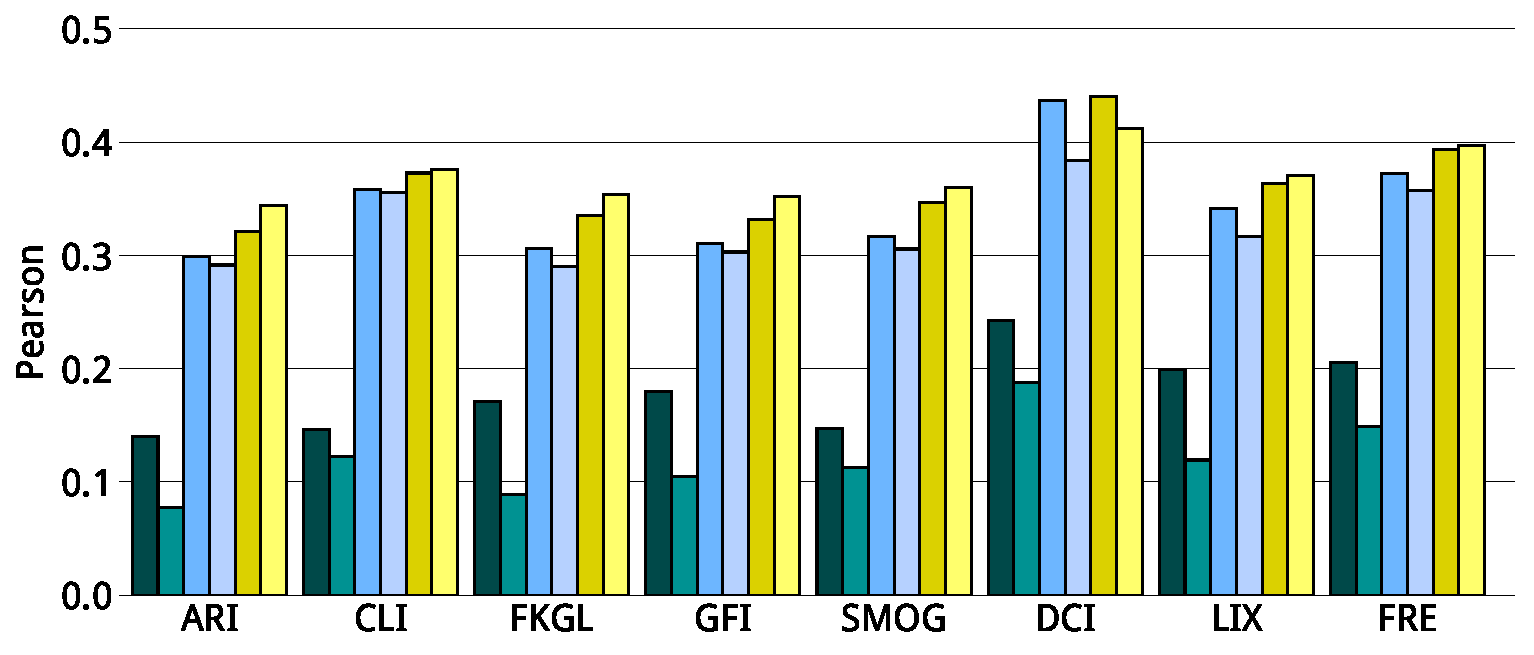
\includegraphics[width=.45\textwidth]{graphics/bar_corr_pearson16_values}
%   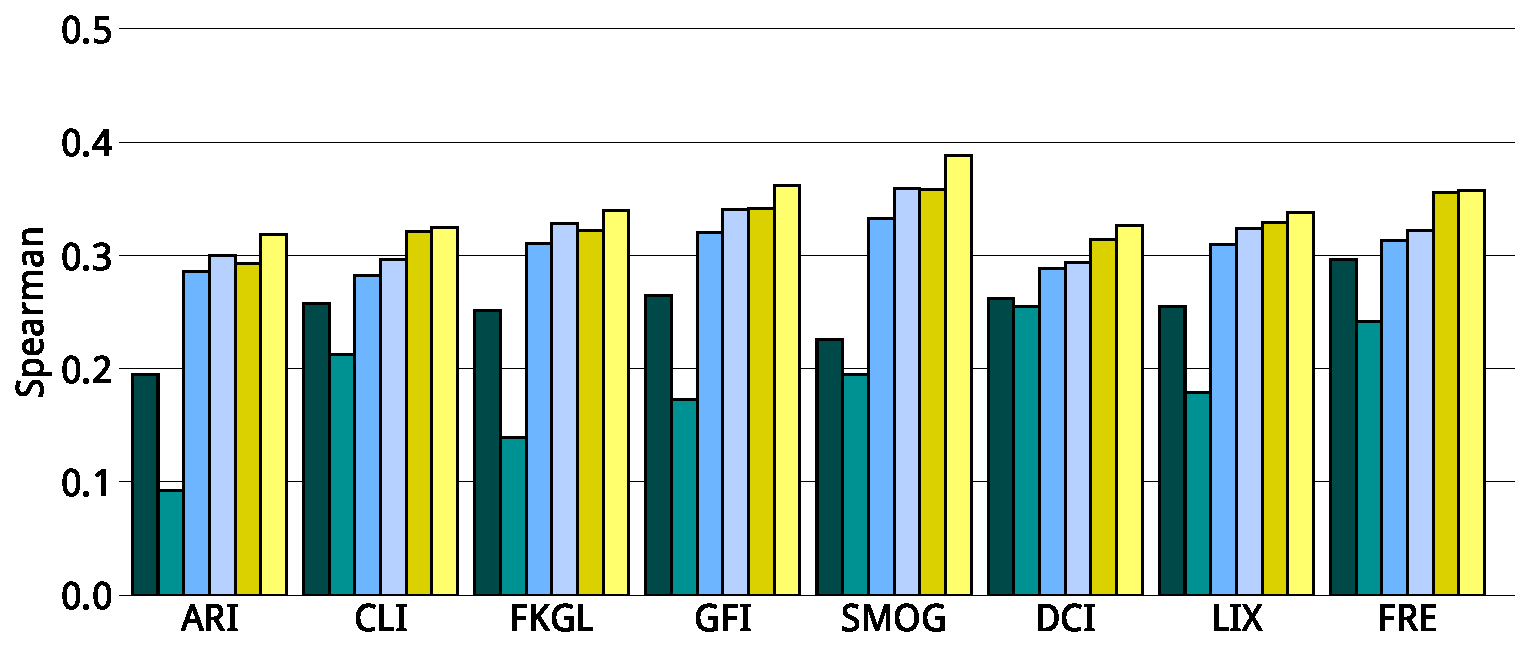
\includegraphics[width=.45\textwidth]{graphics/bar_corr_spearman15_values}
%   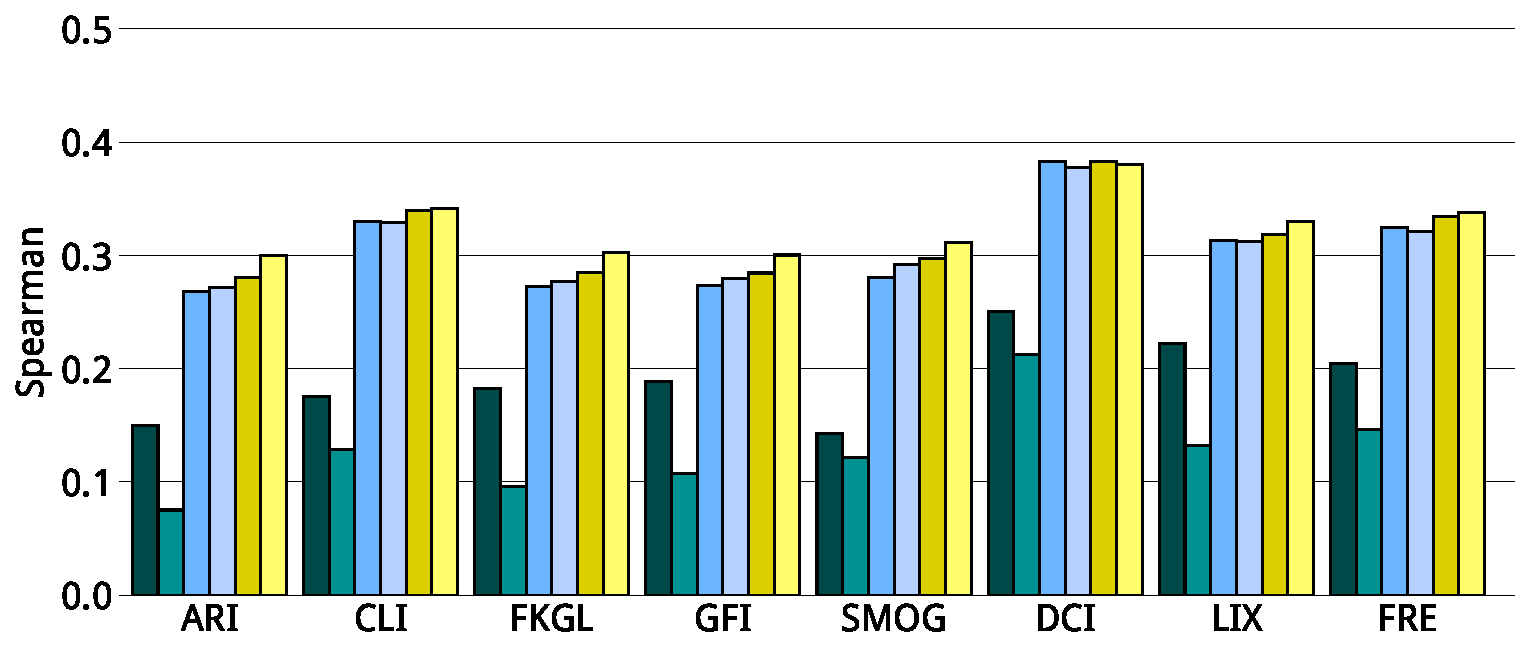
\includegraphics[width=.45\textwidth]{graphics/bar_corr_spearman16_values}
%   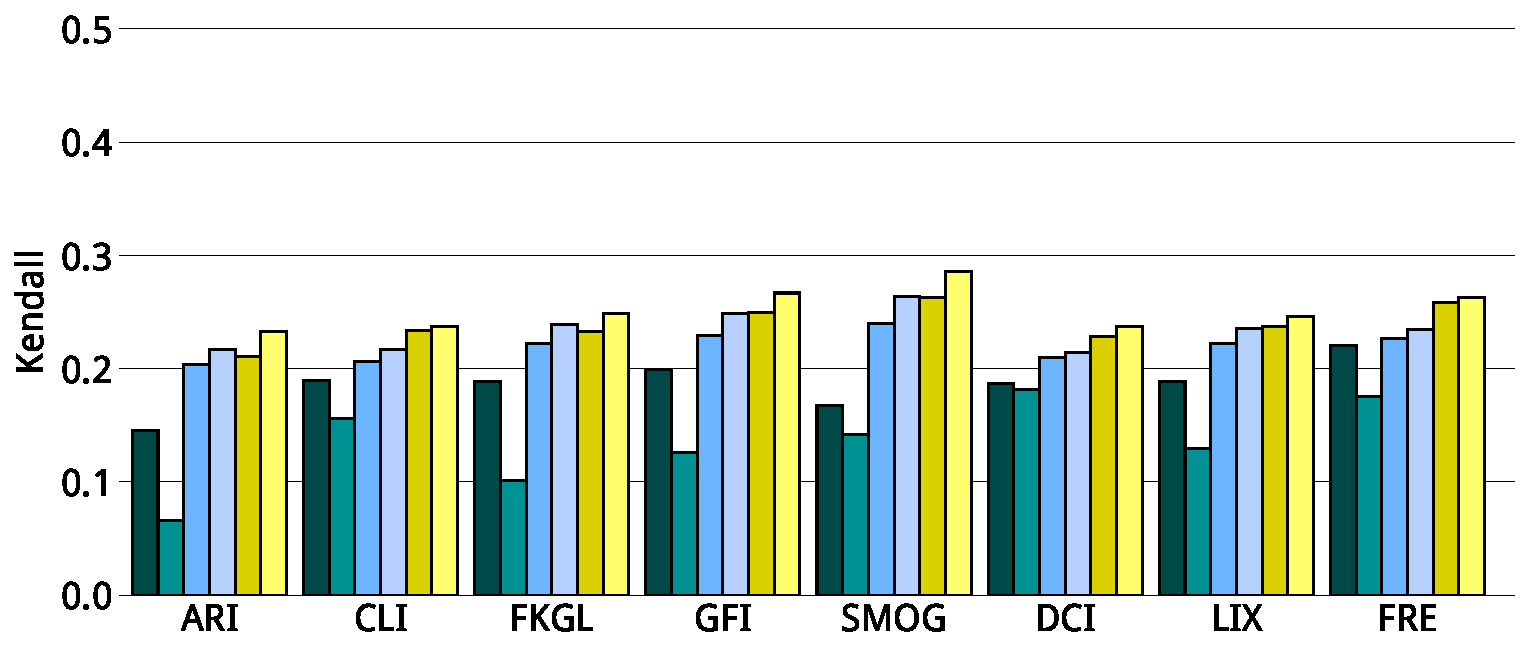
\includegraphics[width=.45\textwidth]{graphics/bar_corr_kendalltau15_values}
%   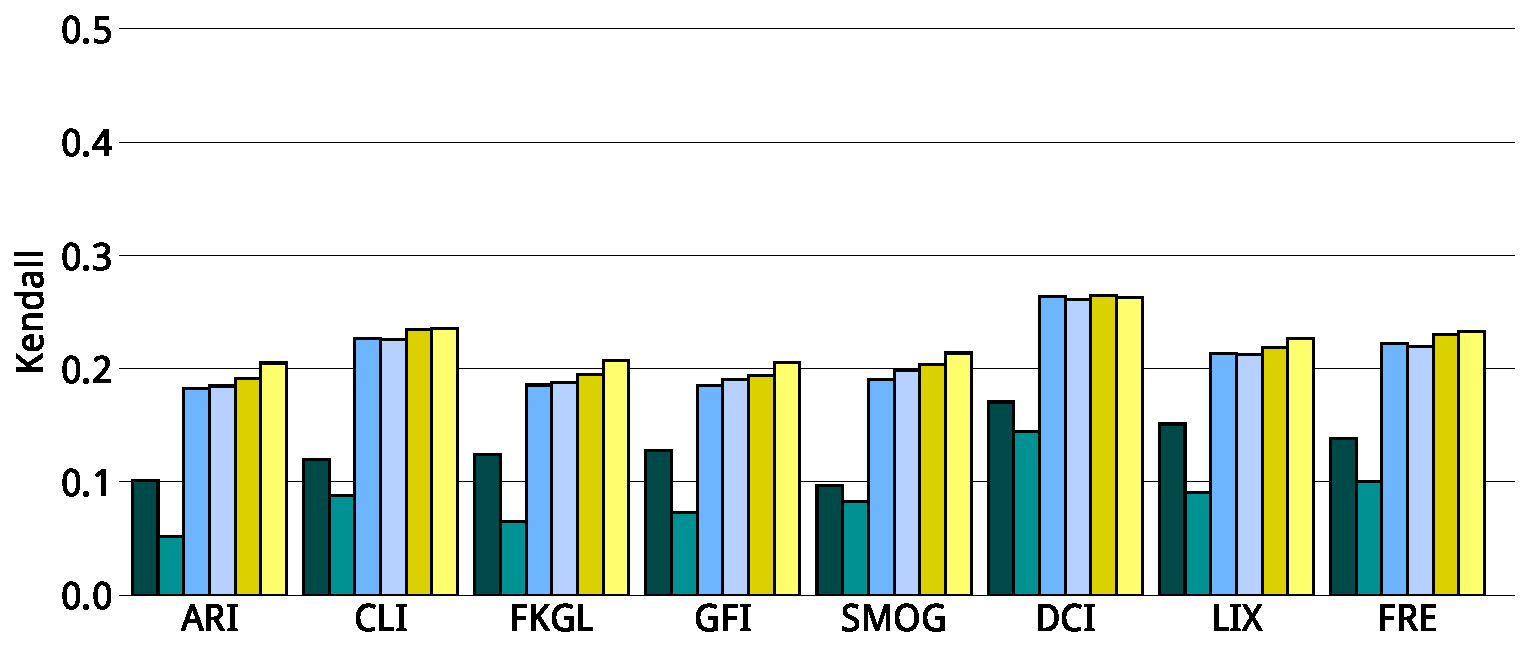
\includegraphics[width=.45\textwidth]{graphics/bar_corr_kendalltau16_values}
%   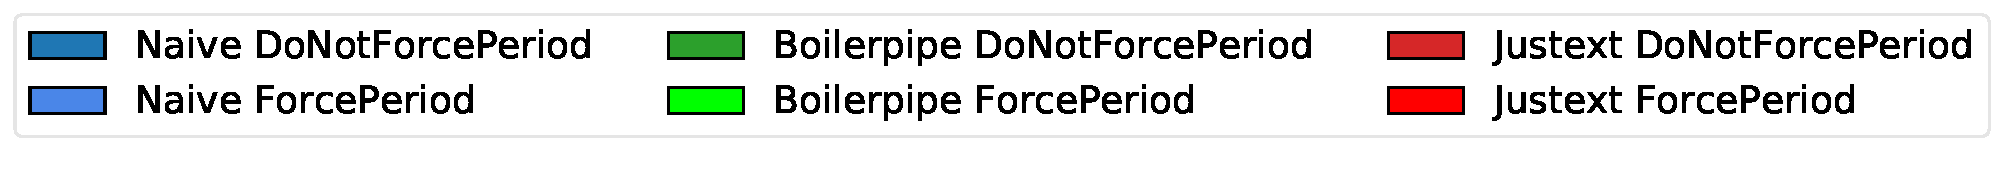
\includegraphics[width=.8\textwidth]{graphics/legend62}
%    \caption{Absolute correlation coefficient of different readability measures and understandability scores. On the left hard side, CLEF eHealth 2015, on the right hand side, CLEF eHealth 2016}
%   \label{fig:bar_corr_clef15}
%\end{figure*}

%\begin{figure*}[th!]
%  \centering
%   \caption{Correlation of different readability measures and the understandability scores collected in CLEF eHealth 2016.}
%  \label{fig:bar_corr_clef16}
%\end{figure*}




\subsection*{Understandability Estimators}
\label{sec:proxies}

%As reviewed in Section~\ref{sec:related}, 
Several methods have been used to estimate the understandability of health Web pages, with the most popular methods (at least in the biomedical literature) being readability formulas based on surface level characteristics of text. Next, we outline the categories of methods to estimate understandability used in this work; an overview is shown in Table~\ref{tab:doc_features}. Some of these methods further expand measures used in the literature. 
 
\begin{table*}[tb]
\caption{Metrics used as understandability proxies; $\star$: raw values are used. $\diamondsuit$: values normalised by number of words in a documents are used. $\dagger$: values normalised by number of sentences in a document are used.}
\label{tab:doc_features}
\resizebox{1.\textwidth}{!}{
\begin{tabular}{llcll}
\cline{1-2} \cline{4-5} 
\textbf{Group} & \textbf{Metric} & \multirow{29}{*}{} & \textbf{Group} & \textbf{Metric}\tabularnewline
\cline{1-2} \cline{4-5} 
\multirow{8}{*}{\textbf{Traditional Readability Formulas}} & Automated Readability Index (ARI) \cite{ari67} &  & \multirow{26}{*}{\textbf{HTML Features}} & \# of Abbr tags\tabularnewline
 & Coleman-Liau Index (CLI) \cite{cli75} &  &  & \# of A tags\tabularnewline
 & Dale Chall Index (DCI) \cite{dale48} &  &  & \# of Blockquote tags\tabularnewline
 & Flesch-Kincaid Grade Level (FKGL) \cite{flesch75} &  &  & \# of Bold tags\tabularnewline
 & Flesch Reading Ease (FRE) \cite{flesch75} &  &  & \# of Cite tags\tabularnewline
 & Gunning Fog Index (GFI) \cite{gunning52} &  &  & \# of Div tags\tabularnewline
 & Lasbarhetsindex (LIX) \cite{lix} &  &  & \# of Forms tags\tabularnewline
 & Simple Measure of Gobbledygook (SMOG) \cite{smog69} &  &  & \# of H1 tags\tabularnewline
\cline{1-2} 
\multirow{10}{*}{\textbf{\makecell{\kern-2.8emRaw Components \\of Readability Measures}}} & \# of Characters $^{\star\diamondsuit\dagger}$ &  &  & \# of H2 tags\tabularnewline
 & \# of Words $^{\star\dagger}$ &  &  & \# of H3 tags\tabularnewline
 & \# of Sentences {$^{\star\diamondsuit}$} &  &  & \# of H4 tags\tabularnewline
 & \# of Difficult Words (Dale Chall list \cite{dale48})
$^{\star\diamondsuit\dagger}$ &  &  & \# of H5 tags\tabularnewline
 & \# of Words Longer than 4 chars $^{\star\diamondsuit\dagger}$ &  &  & \# of H6 tags\tabularnewline
 & \# of Words Longer than 6 chars $^{\star\diamondsuit\dagger}$ &  &  & \# of Hs (any H above)\tabularnewline
 & \# of Words Longer than 10 chars $^{\star\diamondsuit\dagger}$ &  &  & \# of Img tags\tabularnewline
 & \# of Words Longer than 13 chars $^{\star\diamondsuit\dagger}$ &  &  & \# of Input tags\tabularnewline
 & \# of Number of Syllables $^{\star\diamondsuit\dagger}$ &  &  & \# of Link tags\tabularnewline
 & \# of Polysyllable Words (>3 Syllables) $^{\star\diamondsuit\dagger}$ &  &  & \# of DL tags\tabularnewline
\cline{1-2} 
\multirow{6}{*}{\textbf{Medical Vocabularies}} & \# of Words with Medical Prefix $^{\star\diamondsuit\dagger}$ &  &  & \# of UL tags\tabularnewline
 & \# of Words with Medical Suffix $^{\star\diamondsuit\dagger}$ &  &  & \# of OL tags\tabularnewline
 & \# of Acronyms $^{\star\diamondsuit\dagger}$ &  &  & \# of List (DL + UL + OL)\tabularnewline
 & \# of ICD Concepts $^{\star\diamondsuit\dagger}$ &  &  & \# of Q tags\tabularnewline
 & \# of Drugbank $^{\star\diamondsuit\dagger}$ &  &  & \# of Scripts tags\tabularnewline
 & \# of Words in medical dict. (OpenMedSpel) $^{\star\diamondsuit\dagger}$ &  &  & \# of Spans tags\tabularnewline
\cline{1-2} 
    \multirow{6}{*}{\textbf{\makecell{\kern-2.5emConsumer Health\\ Vocabulary (CHV) \cite{zeng06} \\ \kern-6.2emFeatures}}} & CHV Mean Score for all Concepts $^{\star\diamondsuit\dagger}$ &  &  & \# of Table tags\tabularnewline
 & \# of CHV Concepts $^{\star\diamondsuit\dagger}$ &  &  & \# of P tags\tabularnewline
\cline{4-5} 
 & CHV Mean Score for Symptom Concepts $^{\star\diamondsuit\dagger}$ &  & \multirow{20}{*}{\textbf{Word Frequency}} & 25th percentil English Wikipedia\tabularnewline
 & \# of CHV Symptom Concepts $^{\star\diamondsuit\dagger}$ &  &  & 50th percentil English Wikipedia\tabularnewline
 & CHV Mean Score for Disease Concepts $^{\star\diamondsuit\dagger}$ &  &  & 75th percentil English Wikipedia\tabularnewline
 & \# of CHV Disease Concepts $^{\star\diamondsuit\dagger}$ &  &  & Mean Rank English Wikipedia\tabularnewline
\cline{1-2} 
\multirow{6}{*}{\textbf{\makecell{\kern-0.3emMedical Subject\\ Headers (MeSH)}}} & \# of MeSH Concepts $^{\star\diamondsuit\dagger}$ &  &  & Mean Rank English Wikipedia - Includes OV\tabularnewline
 & Average Tree of MeSH Concepts $^{\star\diamondsuit\dagger}$ &  &  & 25th percentil Medical Reddit\tabularnewline
 & \# of MeSH Symptom Concepts $^{\star\diamondsuit\dagger}$ &  &  & 50th percentil Medical Reddit\tabularnewline
 & Average Tree of MeSH Symptom Concepts $^{\star\diamondsuit\dagger}$ &  &  & 75th percentil Medical Reddit\tabularnewline
 & \# of MeSH Disease Concepts $^{\star\diamondsuit\dagger}$ &  &  & Mean Rank Medical Reddit\tabularnewline
 & Average Tree of MeSH Disease Concepts $^{\star\diamondsuit\dagger}$ &  &  & Mean Rank Medical Reddit ncludelude OV\tabularnewline
\cline{1-2} 
\multirow{20}{*}{\textbf{Natural Language}} & Positive Words $^{\star\diamondsuit\dagger}$ &  &  & 25th percentil Pubmed\tabularnewline
 & Negative Words $^{\star\diamondsuit\dagger}$ &  &  & 50th percentil Pubmed\tabularnewline
 & Neutral Words $^{\star\diamondsuit\dagger}$ &  &  & 75th percentil Pubmed\tabularnewline
 & \# of verbs $^{\star\diamondsuit\dagger}$ &  &  & Mean Rank Pubmed\tabularnewline
 & \# of nouns $^{\star\diamondsuit\dagger}$ &  &  &  Mean Rank Pubmed - Includes OV\tabularnewline
 & \# of pronouns $^{\star\diamondsuit\dagger}$ &  &  & 25th p. Wikipedia+Reddit+Pubmed  \tabularnewline
 & \# of adjectives $^{\star\diamondsuit\dagger}$ &  &  & 50th p. Wikipedia+Reddit+Pubmed \tabularnewline
 & \# of adverbs $^{\star\diamondsuit\dagger}$ &  &  & 75th p. Wikipedia+Reddit+Pubmed \tabularnewline
 & \# of adpositions $^{\star\diamondsuit\dagger}$ &  &  & Mean R. Wiki.+Reddit+Pubmed \tabularnewline 
 & \# of conjunctions $^{\star\diamondsuit\dagger}$ & &  & Mean R. Wiki.+Reddit+Pubmed - w. OV \tabularnewline
\cline{4-5} 
 & \# of determiners $^{\star\diamondsuit\dagger}$ & & \multirow{5}{*}{\textbf{Regressor}} & Linear Regressor\tabularnewline  
 & \# of cardinal numbers $^{\star\diamondsuit\dagger}$ &  &  & Gradient Boosting Regressor\tabularnewline
 & \# of particles or other function words $^{\star\diamondsuit\dagger}$ &  &  & Multi-layer Perceptron Regressor\tabularnewline
 & \# of other POS (foreign words, typos) $^{\star\diamondsuit\dagger}$ &  &  & Random Forest Regressor\tabularnewline
 & \# of punctuation $^{\star\diamondsuit\dagger}$ &  &  & Support Vector Machine Regressor\tabularnewline
\cline{4-5} 
 & Height of part-of-speech parser tree $^{\star\diamondsuit\dagger}$ &  &  \multirow{6}{*}{\textbf{Classifier}} & Logistic Regression\tabularnewline
 & \# of Entities $^{\star\diamondsuit\dagger}$ &  &  & Gradient Boosting Classifier\tabularnewline
 & \# of Stopwords $^{\star\diamondsuit\dagger}$ &  &  & Multinomial Naive Bayes\tabularnewline
 & \# of words not found in Aspell Eng. dict. $^{\star\diamondsuit\dagger}$ &  &  & Multi-layer Perceptron Classifier\tabularnewline
 &  &  &  & Random Forest Classifier\tabularnewline
 &  &  &  & Support Vector Machine Classifier\tabularnewline
\cline{1-2} \cline{4-5} 
\end{tabular}
}
\end{table*}


\textit{Traditional Readability Formulas (RF):}
%These include the readability formulas mentioned in Section~\ref{sec:related}, as well as other, less popular ones. A full list is provided in surveys by Collins-Thompson \cite{collins2014computational} and Dubay~\cite{dubay04}.
These include the most popular readability formulas~\cite{cli75,dale48,flesch75}, as well as other, less popular ones~\cite{ari67,gunning52,lix,smog69}. A full list is provided in surveys by Collins-Thompson \cite{collins2014computational} and Dubay~\cite{dubay04}.

\textit{Raw Components of Readability Formulas (CRF):}
These are formed by the ``building blocks'' used in the traditional readability formulas; examples of such building blocks include the average number of characters per word and the average number of syllables in a sentence. Words are divided into syllables using the Python package Pyphen~\cite{pyphen}.

\textit{General Medical Vocabularies (GMV):}
These include methods that count the number of words with a medical prefix or suffix, i.e. beginning or ending with Latin or Greek particles (e.g., amni-, angi-, algia-, arteri-), and text strings included in lists of acronyms or in medical vocabularies such as the International Statistical Classification of Diseases and Related Health Problems (ICD), Drugbank and the OpenMedSpel dictionary~\cite{openmedspel}. An acronym list from the ADAM database~\cite{zhou2006} was used. Methods in this category were matched with documents using simple keywords matching. An acronym list from the ADAM database~\cite{zhou2006} was used and methods in this group were matched with documents using simple keywords matching.

\textit{Consumer Medical Vocabulary (CMV):}
The popular MetaMap \cite{aronson10} tool was used to map the text content of Web pages to entries in  CHV~\cite{zeng06}.
We used the MetaMap semantic types to retain only concepts identified as symptoms or diseases. Similar approaches have been commonly used in the literature (e.g.,~\cite{pang16,agrafiotesA16,palotti16,yates13}).

\textit{Expert Medical Vocabulary (EMV):}
Similarly to the CHV features, we used MetaMap to convert the content of Web pages into MeSH entities, studying symptom and disease concepts separately. 

\textit{Natural Language Features (NLF):}
These included commonly used natural language heuristics such as the ratio of part-of-speech (POS) classes, the height of the POS parser tree, the number of entities in the text, 
the sentiment polarity and the ratio of words found in English vocabularies. The Python package NLTK~\cite{nltk} was employed for sentiment analysis, POS tagging and entity recognition. The GNU Aspell~\cite{aspell} dictionary was used as a standard English vocabulary and a stop word list was built by merging those of Indri~\cite{indri} and Terrier~\cite{terrier}. Discourse features, such as the distribution of POS classes and density of entity in a text, were previously studied in the task of understandability prediction~\cite{feng10} yielding being superior to complex features such as entity co-reference and entity grid (\cite{barzilay08}). To the best of our knowledge, sentiment polarity were never investigated. Our intuition is that laypeople produced content (patient forums or blogs) might content a larger number of emotional content, whereas scientific publications might not

\textit{HTML Features (HF):}
These included the identification of a large number of HTML tags, which were extracted with the Python library BeautifulSoap~\cite{bs4}. The intuition for these features is that Web pages with many images and tables may explain and summarise health content better, thus providing more understandable content to the general public. 

\textit{Word Frequency Features (WFF):}
Generally speaking, common and known words are usually frequent words, while unknown and obscure words are generally rare. This idea  is implemented in readability formulas such as the DCI, which uses a list of common words and counts the number of words that fall outside this list (complex words)~\cite{dale48} and has shown success in other recent approaches~\cite{elhadad06,wu15}.
We extended these observations by studying corpus-wide word frequencies. 
We modelled word frequencies in a corpus in a straightforward manner: we sorted the word frequencies and normalized word rankings such that values close to 100 are attributed to common words and values close to 0 to rare words. Three corpora were analysed to extract word frequencies:

\begin{itemize}[leftmargin=*]
    \item \underline{Medical Reddit:} Reddit~\cite{reddit} is a Web forum with a sizeable user community which is responsible for generating and moderating its content. Any user can start a discussion or reply to a discussion. This forum is intensively used for health purposes: for example in the Reddit community AskDocs~\cite{redditaskdocs}, licensed nurses and doctors (subject to user identity verification) advise help seekers free of charge. We selected six of such communities
        (medical, AskDocs, AskDoctorSmeeee, Health, WomensHealth, Mens\_Health) and downloaded all user interactions available until September 1st 2017 using the Python library PRAW~\cite{redditapi}. In total 43,019 discussions were collected.

\item \underline{Medical English Wikipedia:} after obtaining a recent Wikipedia dump~\cite{wikipedia} (May 1st 2017), we filtered articles to only those containing an Infobox in which at least one of the following words appeared as a property: ICD10, ICD9, DiseasesDB, MeSH, MeSHID, MeshName, MeshNumber, GeneReviewsName, Orphanet, eMedicine, MedlinePlus, drug\_name, Drugs.com, DailyMedID, LOINC. A Wikipedia infobox is a structured template that appears on the right of Wikipedia pages summarizing key aspects of articles.
%Figure~\ref{fig:hyperthermia} illustrates a Wikipedia page that is marked as medical because of its Infobox entries.
This process followed the method by Soldaini et al.~\cite{soldaini15}, which favours precision over recall when identifying a health-related article. This resulted in a collection of 11,868 articles. 
%Note that this procedure highly favors precision over recall. %\mytodo{In case we need space, I suggest we drop this figure}

\item \underline{PubMed Central:} PubMed Central~\cite{pubmed} is an online  database of biomedical literature. We used the collection distributed for the TREC 2014 and 2015 Clinical Decision Support Track~\cite{roberts16,trec15}, consisting of 733,191 articles. 
 
\end{itemize}

A summary of the statistics of these three collections is reported in Table~\ref{tab:collection_stats}. 
%We removed words that occurred less than 5 times in a corpus.  %% We include this detail if necessary in the final version of this paper
%Finally, 
Unless explicitly stated otherwise, we ignored out of vocabulary words in our feature calculations.

%\begin{figure}[th!]
%   \centering
%   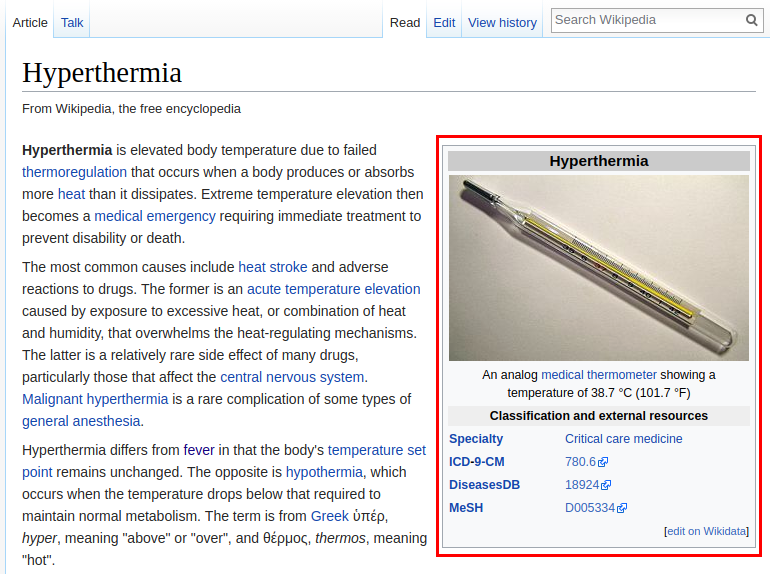
\includegraphics[width=0.50\textwidth]{graphics/hyperthermia}
%    \caption{Wikipedia page on hyperthermia. A rectangular red box identify the Infobox on the right hand side containing entries for Specialty, ICD-9-CM, DiseasesDB and MeSH.}
%    \label{fig:hyperthermia}
%\end{figure}

\begin{table}[!tb]
\centering    
\caption{Statistics for the collections used as background models for understandability estimations.}
\vspace{-0.3cm}
\label{tab:collection_stats}
\resizebox{0.4\textwidth}{!}{
\begin{tabular}{cccc}
\toprule 
\textbf{Statistic} & \textbf{Medical Wikipedia} & \textbf{Medical Reddit} & \textbf{PubMed Central}\tabularnewline
\midrule 
\textbf{Number of Docs.} & 11,868 & 43,019 & 733,191\tabularnewline
\textbf{Number of Words} & 10,655,572 & 11,978,447 & 144,024,976\tabularnewline
\textbf{Number of Unique Words} & 467,650 & 317,106 & 2,933,167\tabularnewline
\textbf{Avg. Words per Doc.} & 898.90 $\pm$ 1351.76 & 278.45 $\pm$ 359.70  & 227.22 $\pm$ 270.44 \tabularnewline
\textbf{Avg. Char per Doc.} & 5107.81 $\pm$ 7618.57  & 1258.44 $\pm$ 1659.96  & 1309.11 $\pm$ 1447.31 \tabularnewline
\textbf{Avg. Char per Word} & 5.68 $\pm$ 3.75  & 4.52 $\pm$ 3.52 &  5.76 $\pm$ 3.51 \tabularnewline
\bottomrule
\end{tabular}
} % End of resizebox
\vspace{-8pt}
\end{table}


\textit{Machine Learning on Text - Regressors (MLR) and Classifiers (MLC):} These include machine learning methods for estimating Web page understandability. While Collins-Thompson highlighted the promise of estimating understandability using machine learning methods, a challenge is identifying the background corpus to be used for training~\cite{collins2014computational}. To this aim, we used the three corpora detailed above, and assumed understandability labels according to the expected difficulty of documents in these collections:

\begin{itemize}[leftmargin=*]
    \item Medical Reddit (label 1): Documents in this collection are expected to be written in a colloquial style, and thus the easiest to understand. All the conversations are in fact explicitly directed to assist inexpert health consumers;
    \item Medical English Wikipedia (label 2): Documents in this collection are expected to be less formal than scientific articles, but more formal than a Web forum like Reddit, thus somewhat more difficult to understand;
    \item PubMed Central (label 3): Documents from this collection are expected to be written in a highly formal style, as the target audience are physicians and biomedical researchers.
\end{itemize}

Models were learnt using all documents from these collections after features were extracted using Latent Semantic Analysis (LSA) with 10 dimensions (this number of dimensions was chosen based on preliminary experiments with the Random Forest algorithm; we leave as future work a detailed study on the impact of different number of dimensions on other machine learning algorithms). We modelled a classification task as well as a regression task using these collections. Thus, after applying the same LSA transformation to test documents from CLEF, a continuous score was assigned to each document by a regressor, while each classifier assigned the documents to one of the three classes. %\footnote{In principle, regressors should output a continuous value between 1 and 3, but no restrictions are set and potentially any value can be assigned to a document.}

%Different labels for the regression could be employed, for example, a label 6 to PubMed Central documents would emphasize that these documents are explicitly made for expert users, being 3 times harder than Wikipedia ones. We did not explore the effects of different labels in this work, it is left as future work.



\subsection{Preprocessing Pipelines and Heuristics}
\label{sec:pipelines}

%As part of our study, we investigated the influence the preprocessing of Web pages has on the estimation of understandability, when this is estimated using the methods in \todo{Section~\ref{sec:proxies}}. 
As part of our study, we investigated the influence the preprocessing of Web pages has on the estimation of understandability, when this is estimated using the methods described above.
We did so by comparing the combination of a number of preprocessing pipelines, heuristics, and understandability estimation methods with human assessments of Web page understandability. 
Our experiments extended those by Palotti et al.~\cite{palotti15} and provided a much thorough analysis, as they only evaluated surface level readability formulas and did not compare their results against human assessments. 
%\mytodo{NEW CONTRIBUTION FOUND...}

To extract the content of a Web page from the HTML source we tested: BeautifulSoup~\cite{bs4} (\textit{Naive}), which just naively removes HTML tags, Boilerpipe~\cite{kohlschutter10} (\textit{Boi}) and Justext~\cite{jan11} ({Jst}), which eliminates boilerplate text together with HTML tags. 
%Palotti et al.'s data analysis highlighted that the text in HTML tags often missed a correct punctuation mark and thus the text extracted from HTML fields like titles, menus, tables and lists could be interpreted as many short sentences or few very long sentences, depending on whether a period was forced at the end of fields/sentences. We thus implement the same two heuristics devised by them to deal with this: \textit{ForcePeriod (FP)} and \textit{DoNotForcePeriod (DNFP)}. The FP heuristic forces a period at the end of each extracted HTML field; while the DNFP does not. 
Palotti et al.'s data analysis highlighted that the text in HTML fields like titles, menus, tables and lists often missed a correct punctuation mark and thus the text extracted from them could be interpreted as many short sentences or few very long sentences, depending on whether a period was forced at the end of fields/sentences. We thus implemented the same two heuristics devised by Palotti et al. to deal with this: \textit{ForcePeriod (FP)} and \textit{DoNotForcePeriod (DNFP)}. The FP heuristic forces a period at the end of each extracted HTML field, while the DNFP does not. 


\subsection{Integrating Understandability into Retrieval}
\label{sec:method_ltr}

% Modified this section to the simple present as we are talking about what we will do in the next section. Next section we use the simple past because we are reporting the experiments that we have already done. I think that is what makes more sense :P  (apart from the fact that changing from past to present we gain some space removing work endings)

%We investigate how understandability estimations could be used and integrated into retrieval methods to increase the quality of search results. We first investigate re-ranking search results from an initial run purely based on understandability estimations. 
We then investigated how understandability estimations can be integrated into retrieval methods to increase the quality of search results. %We start by evaluating re-ranking search results purely basing on understandability estimations. 
Specifically, we considered three retrieval methods of differing quality for the initial retrieval. These included the best two runs submitted to each CLEF task, and a plain BM25 baseline (default Terrier parameters: $b=0.75$ and $k1=1.2$). As understandability estimators we used the eXtreme Gradient Boosting (XGB) regressor~\cite{chen16}, as well as SMOG for CLEF 2015 and DCI for CLEF 2016. These were the best performing approaches \todo{from Section~\ref{sec:beyond_readability}}. Note that for XGB, for assessed documents we used 10-fold cross validation, training XGB on 90\% of the data, and used its predictions for the remaining 10\%. For unassessed documents, we trained XGB on all assessed data, and applied this model to generate predictions. Different machine learning methods and feature selection schemes were experimented with; results are available in the online appendix. XGB was selected because its results were the best, although other methods followed similar trends.


To integrate understandability estimators into the retrieval process, we first investigated \textit{re-ranking} search results retrieved by the initial runs purely based on the understandability estimations. 
If all the search results from a run were to be considered, then such a re-ranking method may place at early ranks Web pages highly likely to be understandable, but possibly less likely to be topically relevant. To balance relevance and understandability, we only re-ranked the first $k$ documents. We explored rank cut-offs $k = 15, 20, 50$. Because evaluation was performed with respect to the first $n=10$ rank positions, the setting $k=15$ provided a conservative re-ranking of search results, while, $k=50$ provided a less conservative re-ranking approach. Results are presented in Section~\ref{results:reranking}.

As an alternative to the previous two-step ranking strategy for combining topical relevance and understandability, we explored the \textit{fusion} of two search results lists separately obtained for relevance and understandability. For this, we used the Reciprocal Rank Fusion (RRF) method~\cite{cormack09}, which was shown effective for combining two lists of search results based on their documents \textit{ranks}, rather than scores. This approach was selected above score-based fusion methods because of the different scoring strategies and distributions employed when scoring for relevance compared to for understandability. For relevance, we used, separately, the three methods used for re-ranking (ECNU~\cite{song15} and KISTI~\cite{oh15} for CLEF2015, GUIR~\cite{soldaini16} and ECNU~\cite{song16} for CLEF 2016, and BM25 for both collections). For understandability, we used, separately, the estimations from SMOG/DCI and XGB. Also for this approach, we studied limiting the ranking of results to be considered by the methods across the cut-offs $k=15, 20, 50$. Results are presented in Section~\ref{results:fusion}.

\begin{table}[!t]
\centering
\caption{Learning to rank settings. }
\vspace{-0.3cm}
\label{tab:ltr}
\resizebox{0.35\textwidth}{!}{
\begin{tabular}{l|l|l}
\toprule 
Name & Feature Set & Labeling Function\tabularnewline
\midrule 
Combo 1 & IR features & F(R,U) = $R$\tabularnewline
Combo 2 & IR + Unders. features & F(R,U) = $R$ \tabularnewline
Combo 3 & IR + Unders. features & F(R,U) = $R \times (100 - U)/100$ \tabularnewline
Combo 4 & IR + Unders. features & F(R,U) = $\begin{cases} R & \text{if } U \le 40\\ 0 & \text{otherwise}  \end{cases}$ \tabularnewline
Combo 5 & IR + Unders. features & F(R,U) = $\begin{cases} 2 \times R & \text{if } U \le 40\\ R & \text{otherwise}  \end{cases}$\tabularnewline
\bottomrule
\end{tabular}
}% end resizebox
\vspace{-14pt}
\end{table}


Finally, we considered a third alternative to combine relevance and understandability: using \textit{learning to rank} with features derived from retrieval methods (IR features) and understandability estimators.
With the CLEF 2016 collection, we explored five combinations of label attribution and feature sets, maintaining the same pairwise learning to rank algorithm based on tree boosting (XGB).
These combinations are listed in Table~\ref{tab:ltr}, with $R$ being the relevance of documents and $U$ their understandability estimation. While the definitions of Combo 1 and 2 are straightforward, the other methods deserve some further explanation. In Combo 3, a penalty was proportionally assigned to documents according to how far their understandability score was from a target score $U$ (we used $U=40$). For example, a document with understandability 100 received no penalty, as 100 was the easiest level of understanding, while another with understandability 50 received a 50\% penalty, meaning that its relevance score was halved. Combo 4 and 5 were based on a fixed threshold applied to the understandability score: if the score was higher than the threshold $U=40$, then the original relevance score (for Combo 4) or a boosted value (for Combo 5) was assigned to the corresponding document.


\subsection{Additional Resources}
%\todo{Move this section to the discussion part?}
In order to keep this article as succinct as possible, we only reported a subset of the results. The remaining results (which show similar trends to those reported here) are made available in an online supplementary appendix for completeness: {\url{https://sites.google.com/view/understandabilityontheweb/}. All data and code will be shared on GitHub upon acceptance.



\section{Evaluation of understandability estimators}
\label{sec:beyond_readability}
Using the CLEF eHealth 2015 and 2016 collections, we studied the correlations of methods to estimate Web page understandability (Table~\ref{tab:doc_features}) and human assessments. For each category of understandability estimation method, Table~\ref{tab:top_corr_metrics} reports the methods with highest Pearson, Spearman or Kendall correlations.

Overall, Spearman and Kendall correlations obtained similar results (in terms of which methods exhibited the highest correlations): this was expected as, unlike Pearson, they are both rank-based correlations.

For surface level readability measures,  the SMOG Index had the highest correlations for CLEF 2015 and Dale-Chall Index for CLEF 2016, regardless of correlation measure. These results resonated with those obtained for the category of raw components of readability formulas. In fact, the polysyllable words measure, which is the main feature used in SMOG, had the highest correlation for CLEF 2015 among these methods. While, the number of difficult words, which is the main feature used in Dale-Chall index, had the highest correlation for CLEF 2016 among these methods.


%We correlated each individual understandability estimator listed in Table~\ref{tab:doc_features} \todo{is it too small?} with the human assessments collected in CLEF eHealth 2015 and 2016 campaigns.
%We report in Table~\ref{tab:top_corr_metrics} the best metric for each group according to Pearson, Spearman or Kendall correlation.

%For some groups, such as the readability formula group, the highest correlated metric was the same for different correlation measure: SMOG Index in CLEF eHealth 2015 and Dale-Chall Index in 2016. 
%We highlight the top score value of each correlation measure in each group. Note that there is no single case in which three different metrics were the top correlated for each different correlation measure.
%\todo{hypotesis that kendatll tau and spearman always point to the same winner}

%Interestingly, Table~\ref{tab:top_corr_metrics} shows that the polysyllable words, best formula component metric for CLEF 2015 data, is the main metric for the SMOG formula, the best readability formula for CLEF 2015. 
%Likewise, the number of difficult words, best formula component metric for CLEF 2016, is the main metric for Dale-Chall index, the best readability formula for CLEF 2016.

When examining the expert vocabulary category, we found that the number of MeSH concepts obtained the highest correlations with human assessments; however its correlations were sensibly lower than those achieved by the best method from the consumer medical vocabularies category, i.e. the scores of CHV concepts. For the natural language category, we found that the number of pronouns, the number of stop words and the number of out of vocabulary words had the highest correlations -- and these were even higher than those obtained with MeSH and CHV based methods. In turn, the methods that obtained the highest correlations among the HTML category (counts of P tags and list tags) exhibited overall the lowest correlations compared to methods in the other categories. P tags are used to create paragraphs in a Web page, being thus a rough proxy for text length. 
Among methods in the word frequency category, the use of Medical Reddit (but also of PubMed) showed the highest correlations, and these were comparable to those obtained by the readability formulas. 


%The top correlation for MeSH group, number of MeSH concepts, reaches much lower correlation than the top correlation metric for the CHV group, the scores of CHV concepts.
%The dominating metrics for the Natural Language group are the number of pronouns, the number of stopwords and the number of out of vocabulary words; all these are consistently more correlated than metrics in the MeSH and CHV group.
%In turn, the top correlations for the HTML group, counts of P tags and list tags, were the weakest. P tags are used to create paragraphs in a Web page, being roughly a proxy for text lengthiness. 

Finally, regressors and classifiers exhibited the highest correlations across all categories: in this  category, the  Neural Network regressor and the multinomial Naive Bayes best correlated with human assessments. \todo{What about the background corpus for training? JP: didnt understand your question...}

\todo{Keep? Remove? The study of the best understandability estimators provides us significant insights that will be further used for reranking results according to their understandability. ????}


%Top estimators for the word frequency group are based on the Medical Reddit and PubMed counts, with correlations as high as the readability formulas.
%Finally, the group with the highest correlated estimators are the regressors and classifiers, with top estimators being the Neural Network regressor and the multinomial Naive Bayes.
%\todo{this section misses some sort of conclusion or at least a link to the next section}
%
\begin{table}[t]
\centering    
\caption{Metrics with highest correlation per group. In bold are the metric that archived the highest correlation for a correlation measure.}
\label{tab:top_corr_metrics}
\resizebox{.45\textwidth}{!}{ %%%%
\begin{tabular}{c|c|c|c|c|c|c}
\toprule
\textbf{Dataset} & \textbf{Group} & \textbf{Metric} & \textbf{Preproc.} & \textbf{Pears.} & \textbf{Spear.} & \textbf{Kend.}\tabularnewline
\midrule
\multirow{15}{*}{CLEF 2015} & RF & SMOG Index & JST NFP & \textbf{0.438} & \textbf{0.388} & \textbf{0.286}\tabularnewline
\cmidrule{2-7} 
 & \multirow{2}{*}{CRF} & Avg. Num. of Polysyl. Words per Word & JST FP & \textbf{0.429} & 0.364 & 0.268\tabularnewline
 &  & Avg. N. of Polysyl. Words per Sentence & JST NFP & 0.192 & \textbf{0.388} & \textbf{0.286}\tabularnewline
\cmidrule{2-7} 
& \multirow{2}{*}{GMV} & Avg. N. Medical Prefixes per Word & Naive FP & \textbf{0.314} & 0.312 & 0.229\tabularnewline
 &  & Number of Medical Prefixes & Naive FP & 0.131 & \textbf{0.368} & \textbf{0.272}\tabularnewline
\cmidrule{2-7} 
 & CMV & CHV Mean Score for all Concepts & Naive FP & \textbf{0.371} & \textbf{0.314} & \textbf{0.228}\tabularnewline
\cmidrule{2-7} 
 & EMV & Number of MeSH Concepts & Naive FP & \textbf{0.227} & \textbf{0.249} & \textbf{0.178}\tabularnewline
\cmidrule{2-7} 
 &  \multirow{2}{*}{NLF} & N. of words not found in Aspell Dict. & JST NFP & \textbf{0.351} & 0.276 & 0.203\tabularnewline
 &  & Number of Pronouns per Word & Naive FP & 0.271 & \textbf{0.441} & \textbf{0.325}\tabularnewline
\cmidrule{2-7} 
 & HF & Number of P Tags & None & \textbf{0.219} & \textbf{0.196} & \textbf{0.142}\tabularnewline
\cmidrule{2-7} 
 &  \multirow{2}{*}{WFF} & Mean Rank Medical Reddit - Includes OV & JST NFP & \textbf{0.435} & 0.277 & 0.197\tabularnewline
 &  & 25th percentil Pubmed & JST NFP & 0.330 & \textbf{0.347} & \textbf{0.256}\tabularnewline
\cmidrule{2-7} 
 &  \multirow{2}{*}{MLR} & Neural Network Regressor & BOI NFP & \textbf{0.602} & 0.394 & 0.287\tabularnewline
 &  & Neural Network Regressor & JST FP & 0.565 & \textbf{0.438} & \textbf{0.324}\tabularnewline
\cmidrule{2-7} 
 & MLC & Multinomial Naive Bayes & Naive FP & \textbf{0.573} & \textbf{0.477} & \textbf{0.416}\tabularnewline
\midrule
\midrule
\multirow{18}{*}{CLEF 2016} & \multirow{2}{*}{RF} & Dale Chall Index & JST FP & \textbf{0.439} & 0.381 & 0.264\tabularnewline
 &  & Dale Chall Index & BOI FP & 0.437 & \textbf{0.382} & \textbf{0.264}\tabularnewline
\cmidrule{2-7} 
 & CRF & Avg. Difficult Words Per Word & BOI FP & \textbf{0.431} & \textbf{0.379} & \textbf{0.262}\tabularnewline
\cmidrule{2-7} 
 & \multirow{2}{*}{GMV} & Avg. Prefixes per Sentence & JST FP & \textbf{0.263} & 0.242 & 0.164\tabularnewline
 &  & ICD Concepts Per Sentence & JST NFP & 0.014 & \textbf{0.253} & \textbf{0.172}\tabularnewline
\cmidrule{2-7} 
 & \multirow{2}{*}{CMV} & CHV Mean Score for all Concepts & JST FP & \textbf{0.329} & 0.313 & 0.216\tabularnewline
 &  & CHV Mean Score for all Concepts & BOI FP & 0.329 & \textbf{0.325} & \textbf{0.224}\tabularnewline
\cmidrule{2-7} 
 & \multirow{2}{*}{EMV} & Number of MeSH Concepts & BOI NFP & \textbf{0.201} & 0.166 & 0.113\tabularnewline
 &  & Number of MeSH Disease Concepts & BOI NFP & 0.179 & \textbf{0.192} & \textbf{0.132}\tabularnewline
\cmidrule{2-7} 
 & \multirow{2}{*}{NLF} & Avg. Stopword Per Word & BOI FP & \textbf{0.344} & 0.312 & 0.213\tabularnewline
 &  & Number of Pronouns & BOI FP & 0.341 & \textbf{0.364} & \textbf{0.252}\tabularnewline
\cmidrule{2-7} 
& \multirow{2}{*}{HF} & Number of Lists & \multirow{2}{*}{None} & \textbf{0.114} & 0.021 & 0.015\tabularnewline
 &  & Number of P Tags &  & 0.110 & \textbf{0.123} & \textbf{0.084}\tabularnewline
\cmidrule{2-7} 
 & \multirow{2}{*}{WFF} & Mean Rank Medical Reddit & BOI NFP & \textbf{0.387} & 0.312 & 0.214\tabularnewline
 &  & 50th percentil Medical Reddit & JST NFP & 0.351 & \textbf{0.315} & \textbf{0.216}\tabularnewline
\cmidrule{2-7} 
 & \multirow{2}{*}{MLR} & Neural Network Regressor & JST NFP & \textbf{0.454} & \textbf{0.373} & 0.258\tabularnewline
 &  & Random Forest Regressor & BOI NFP & 0.389 & 0.355 & \textbf{0.264}\tabularnewline
\cmidrule{2-7} 
 & MLC & Multinomial Naive Bayes & JST FP & \textbf{0.461} & \textbf{0.391} & \textbf{0.318}\tabularnewline
\bottomrule
\end{tabular}
} %%%%% ---- 
\end{table}

%



\section{Preprocessing Pipelines and Heuristics}

%\section{Which Preprocessing Approach To Prefer}
Next, we studied the influence of the preprocessing of Web pages on the estimation of understandability when using the methods evaluated in the previous section. We did so by comparing the combination of a number of pre-processing pipelines, heuristics and understandability estimation methods with human assessments of web page understandability. 
Our experiments extended those by Palotti et al.~\cite{palotti15}, who did only evaluate surface level readability formulas and did not compare their results against human assessments. 

We employed the same three approaches used in Palotti et al.~\cite{palotti15} to extract the content of a Web page from the HTML source: BeautifulSoap~\cite{bs4} (\textit{Naive}), which just naively removes HTML tags, Boilerpipe~\cite{kohlschutter10} (\textit{Boilerpipe - Boi}) and Justext~\cite{jan11} ({Justext - Jst}), which eliminate boilerplate text together with HTML tags. 
Their data analysis highlighted that the text in HTML tags often missed a correct punctuation mark and thus the text extracted from HTML fields like titles, menus, tables and lists could be interpreted as many short sentences or few very long sentences, depending on whether a period was forced at the end of fields/sentences. We thus implemented the same two heuristics to deal with this: \textit{ForcePeriod - FP} and \textit{DoNotForcePeriod - DNFP}. The \textit{ForcePeriod - FP} heuristics forced a period at the end of each extracted HTML field; while the \textit{DoNotForcePeriod - DNFP} did not. 


\section{Evaluation of Preprocessing Pipelines and Heuristics}
\label{sec:which_preprocessing}
Results from these experiments are shown in Figure~\ref{fig:boxplot_corr_docs} (top: CLEF 2015; bottom: CLEF 2016). For each category of methods and combination of preprocessing and heuristics, we reported their variability in Spearman rank correlation with the human assessments\footnote{Results for Pearson and Kendall correlation measures are reported in the online appendix, but showed similar trends.}. We further reported summary results across all understandability assessments methods and sentence ending heuristics for each of the preprocessing pipelines. Finally, we also reported the inter-assessor correlation (last box) when multiple assessors provided judgements about the understandability of Web pages (see Section~\ref{sec:data} for details about this data). This provided an indication of the range of variability and subjectiveness when assessing understandability, along with the highest correlation we measured between human assessors. 

We first examined the correlations between human assessments and readability formulas. We found that the \textit{Naive} preprocessing resulted in the lowest correlations, regardless readability formula and heuristics (although \textit{DoNotForcePeriod} performed better than \textit{ForcePeriod}). Using Justext or Boilerplate resulted in higher correlations with human understandability assessments, and the \textit{ForcePeriod} heuristic was shown to be better than the other. These results confirm the speculations of Palotti et al.~\cite{palotti15}: they found these settings to produce lower variances in understandability estimations and thus hypothesise they were better suited to the task.

Overall, among readability formulas, the best results (highest correlations) were obtained by SMOG and Dale-Chall Index (see Table~\ref{tab:top_corr_metrics}). Although no single setting outperformed the others in both collections, we found that the use of CLI and FRE with \textit{Justext} provided the most stable results across the collections, with correlation coefficients as high as the best ones in both collections.
These results confirmed the advice put forward by Palotti et al.~\cite{palotti15}, i.e. if using readability measures, then CLI should be preferred, along with an appropriate HTML extraction pipeline, regardless of the heuristic for sentence ending\footnote{We provide detailed plots to compare our results with Palotti's in the online appendix.}.

When considering methods beyond those based on readability formulas, we found that the highest correlations were archived by the regressors (MLR) and classifiers (MLC), independently of the preprocessing method used. For methods in these categories, correlations were only marginally influenced by preprocessing and heuristics, with the exception for regressors on CLEF 2015 that did exhibit not negligible variances. \todo{I think the text is not clear here: need to discuss.} 

A common trend when comparing preprocessing pipelines, is that the Naive pipeline provided the weakest correlations with human assessments for CLEF 2016, regardless of estimation methods and heuristics. This result however was not confirmed for CLEF 2015, where the Naive preprocessing did negatively influence correlations for the readability formula category (RF), but not for other categories, although it was generally associated with larger variances. 


%For that, we present in Figure~\ref{fig:boxplot_corr_docs} the box plot of Spearman rank correlation metric divided by preprocessing alternative for CLEF eHealth 2015 and 2016\footnote{Due to space limitation, additional plots with Pearson and Kendall correlations are available online at \url{XYZ}.}.
%Figures~\ref{fig:boxplot_corr_docs_2015} and~\ref{fig:boxplot_corr_docs_2016} the box plot of different correlation metrics divided by preprocessing alternative for CLEF eHealth 2015 and 2016. 
%For instance, the very first box plot in the upper part of these figures shows the absolute Pearson's rank correlation of different readability metrics when using a combination of Naive and ForcePeriod as preprocessing steps.
%Boxes extend from the lower to upper quartile values of the data, with a line at the median. Whiskers extend from the box to show the range of the data. Flier points are those past the end of the whiskers, usually interpreted as outlier values.




%We also include in Figures~\ref{fig:boxplot_corr_docs_2015} and~\ref{fig:boxplot_corr_docs_2016} 
%We also include in Figure~\ref{fig:boxplot_corr_docs} boxes for the summary of the 3 preprocessing procedures to remove HTML, the use of HTML features, which is done without any preprocessing and the comparison with other human assessors. For CLEF eHealth 2015, we used as human assessments the additional assessments made by unpaid medical students and health consumers (see~\cite{palotti16b}), while for CLEF eHealth 2016 data, we randomly selected 100 pages that were assessed by another assessor. \mytodo{add at least another person doing assessments}.
%The correlations with human assessments provide important insights on how hard and subjective understandability assessments are.

\begin{figure*}[h!]
   \centering
   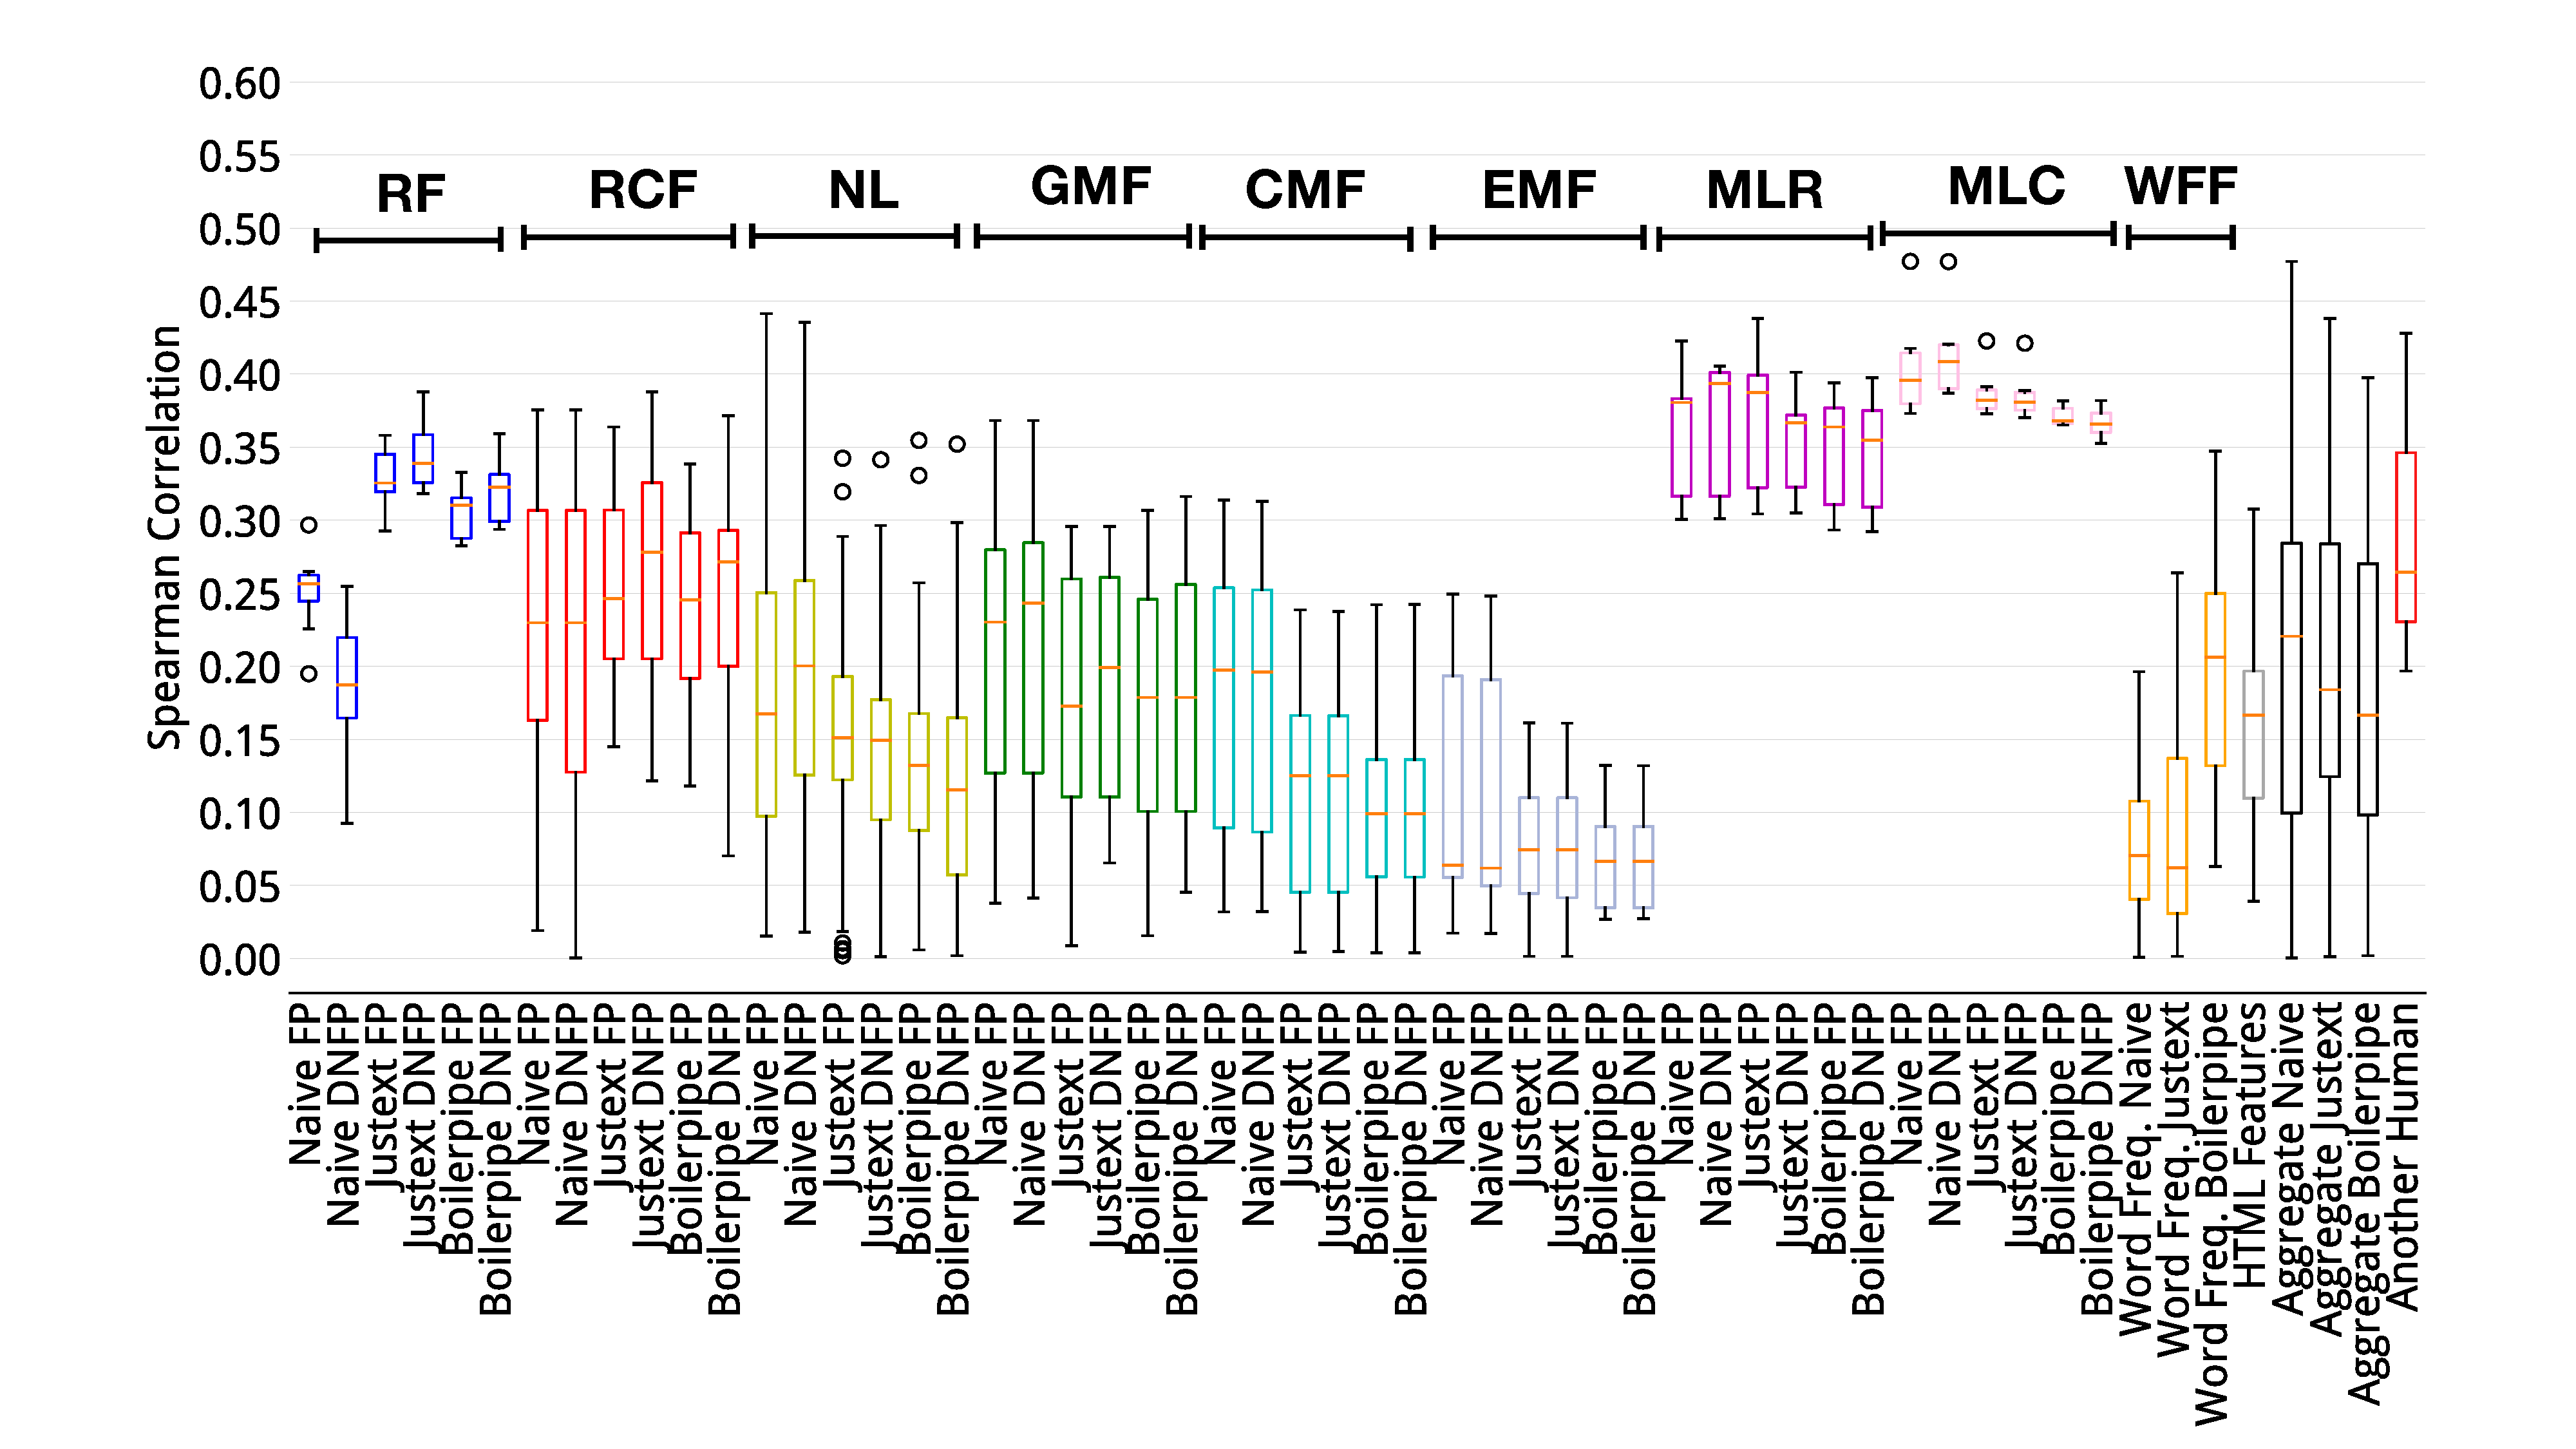
\includegraphics[width=0.80\textwidth]{graphics/box_spearman15_raw_values_mod}
   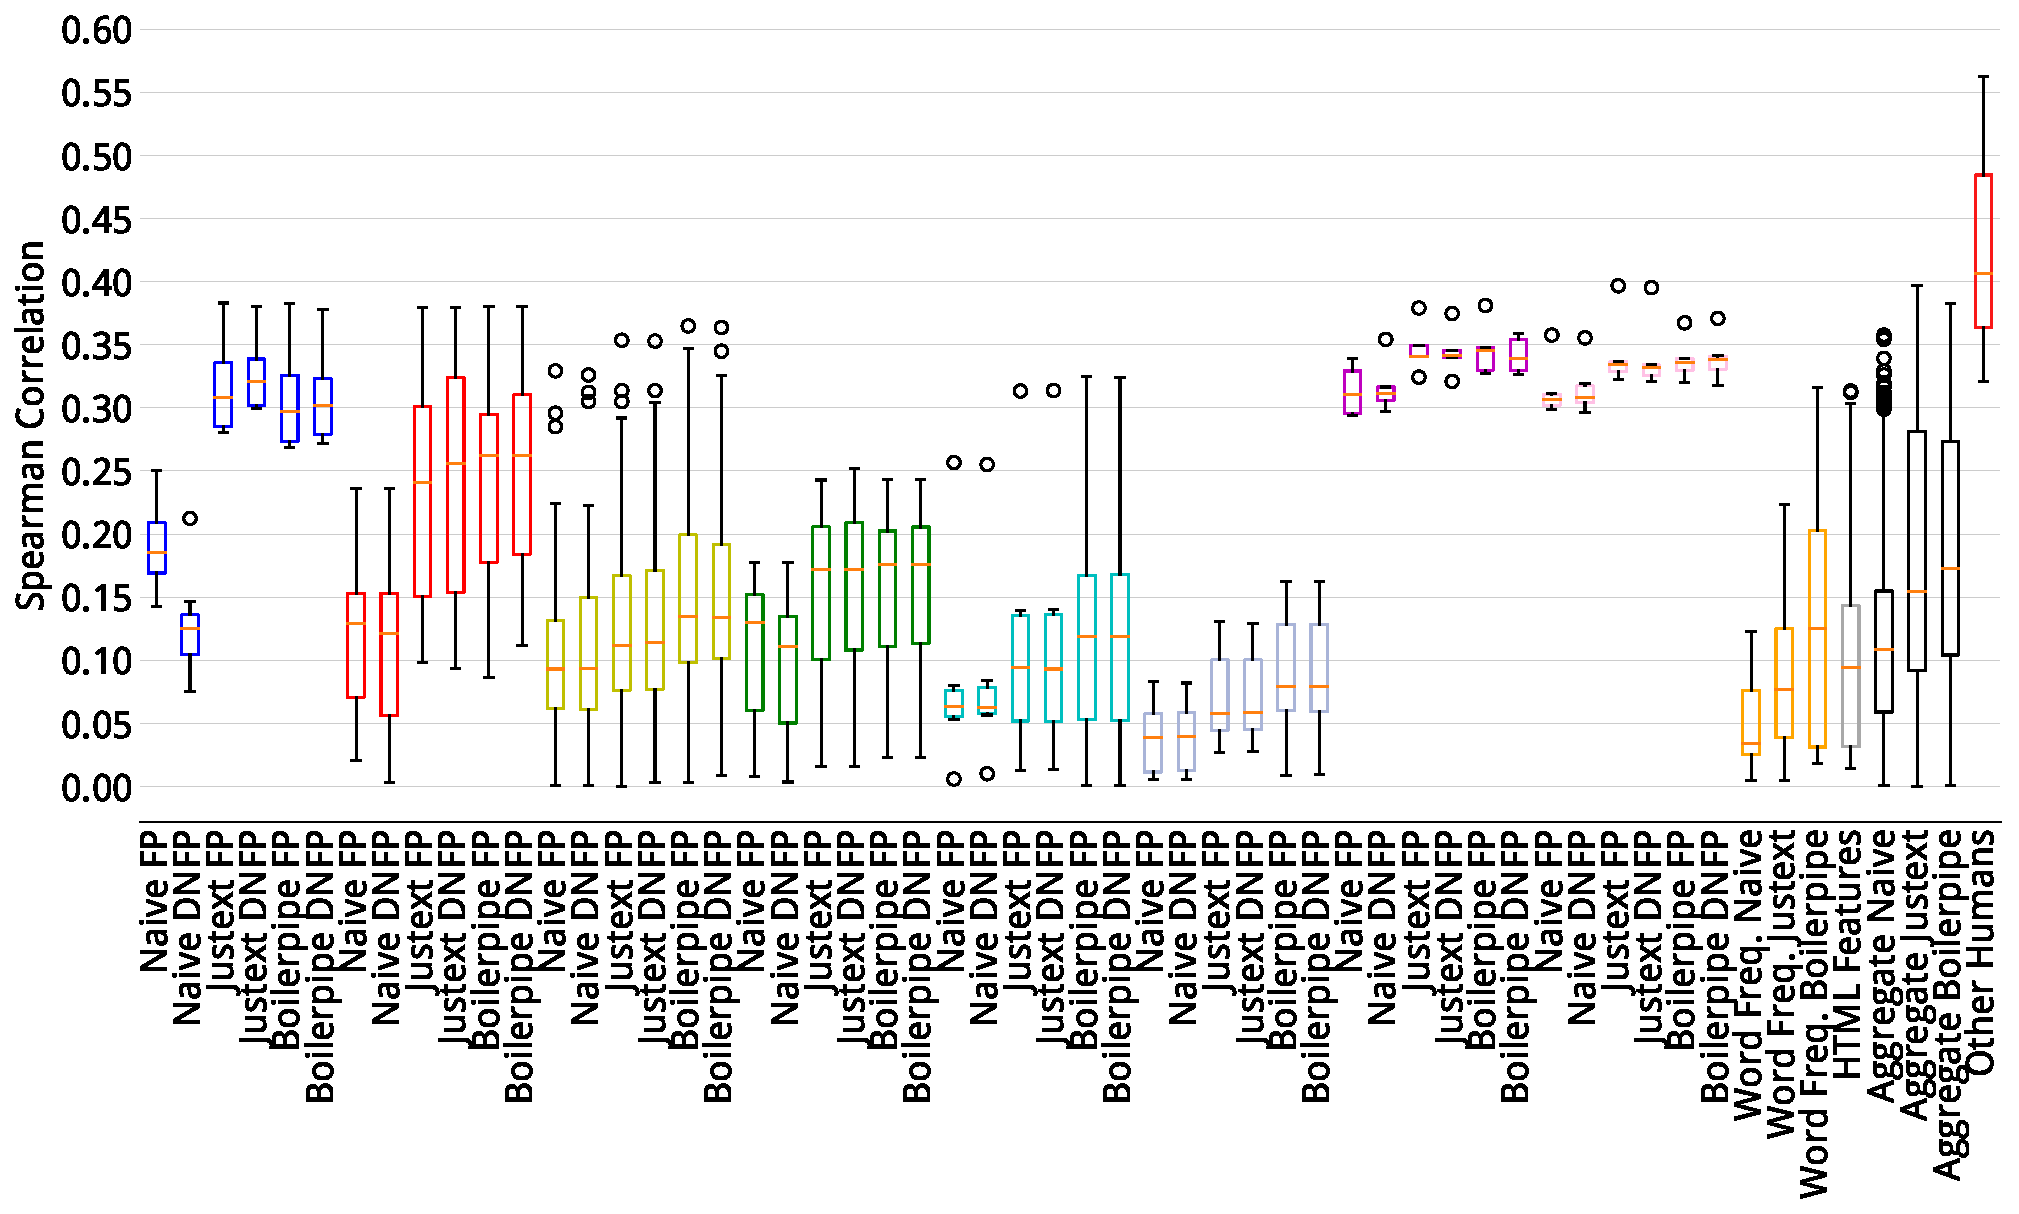
\includegraphics[width=0.80\textwidth]{graphics/box_spearman16_raw_values}
   %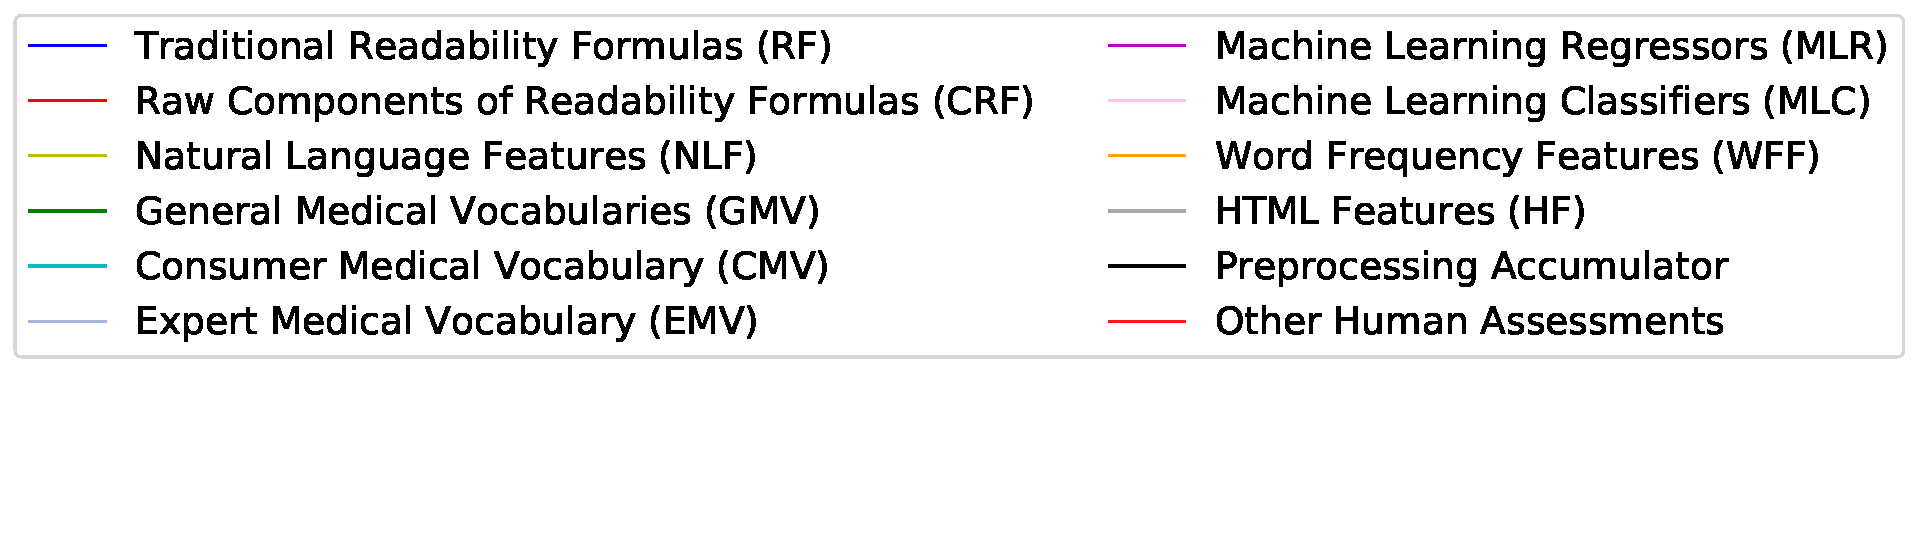
\includegraphics[width=0.7\textwidth]{graphics/legendCorr}
   \vspace{-1cm}
   \caption{Box plots divided by feature groups. Correlations are calculated using understandability labels from relevant documents assessed in CLEF eHealth 2015 (top) and 2016 (bottom).}
   \label{fig:boxplot_corr_docs}
\end{figure*}

%
%\begin{figure*}[th!]
%   \centering
%   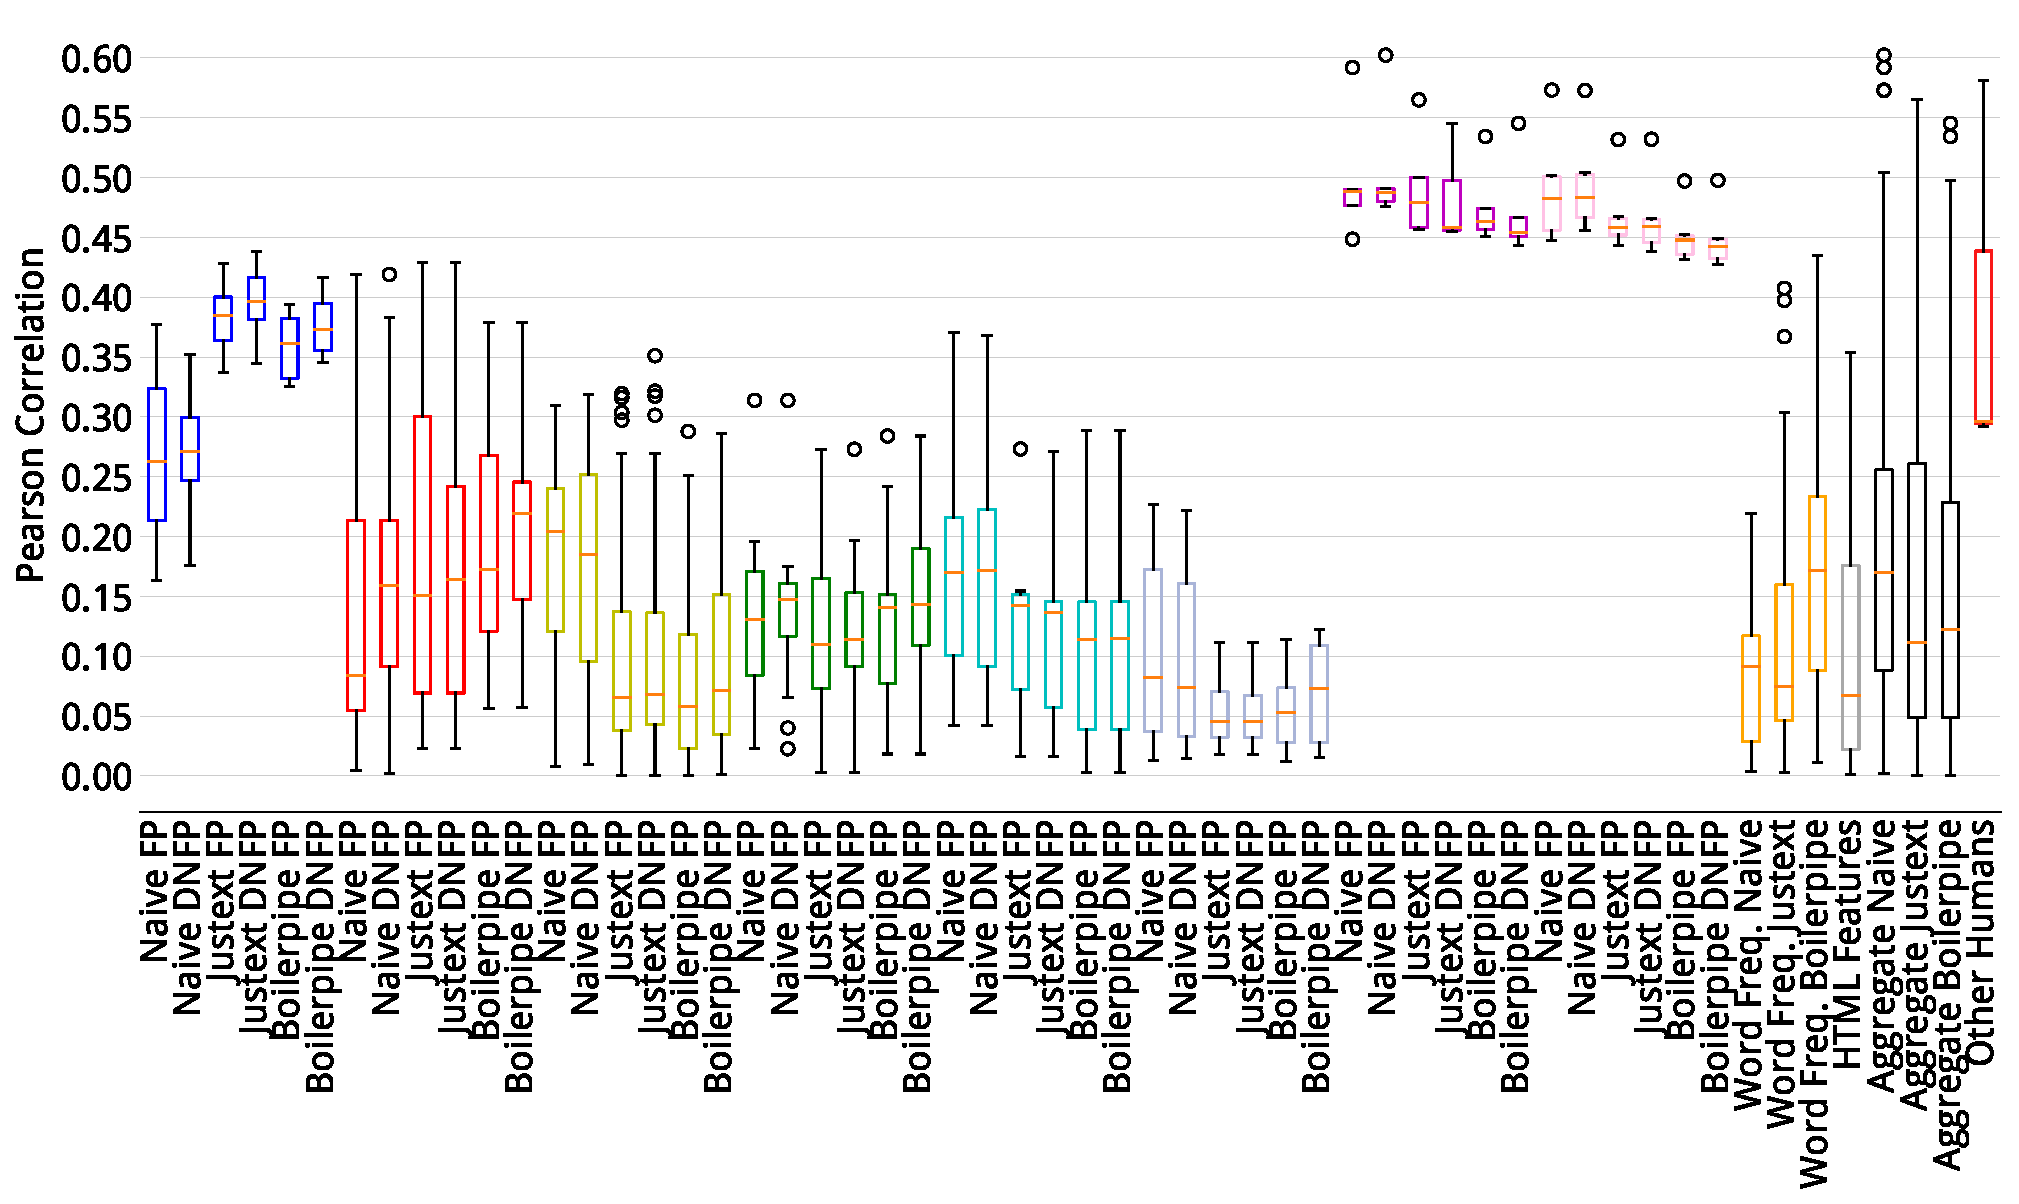
\includegraphics[width=0.90\textwidth]{graphics/box_pearson15_raw_values}
%   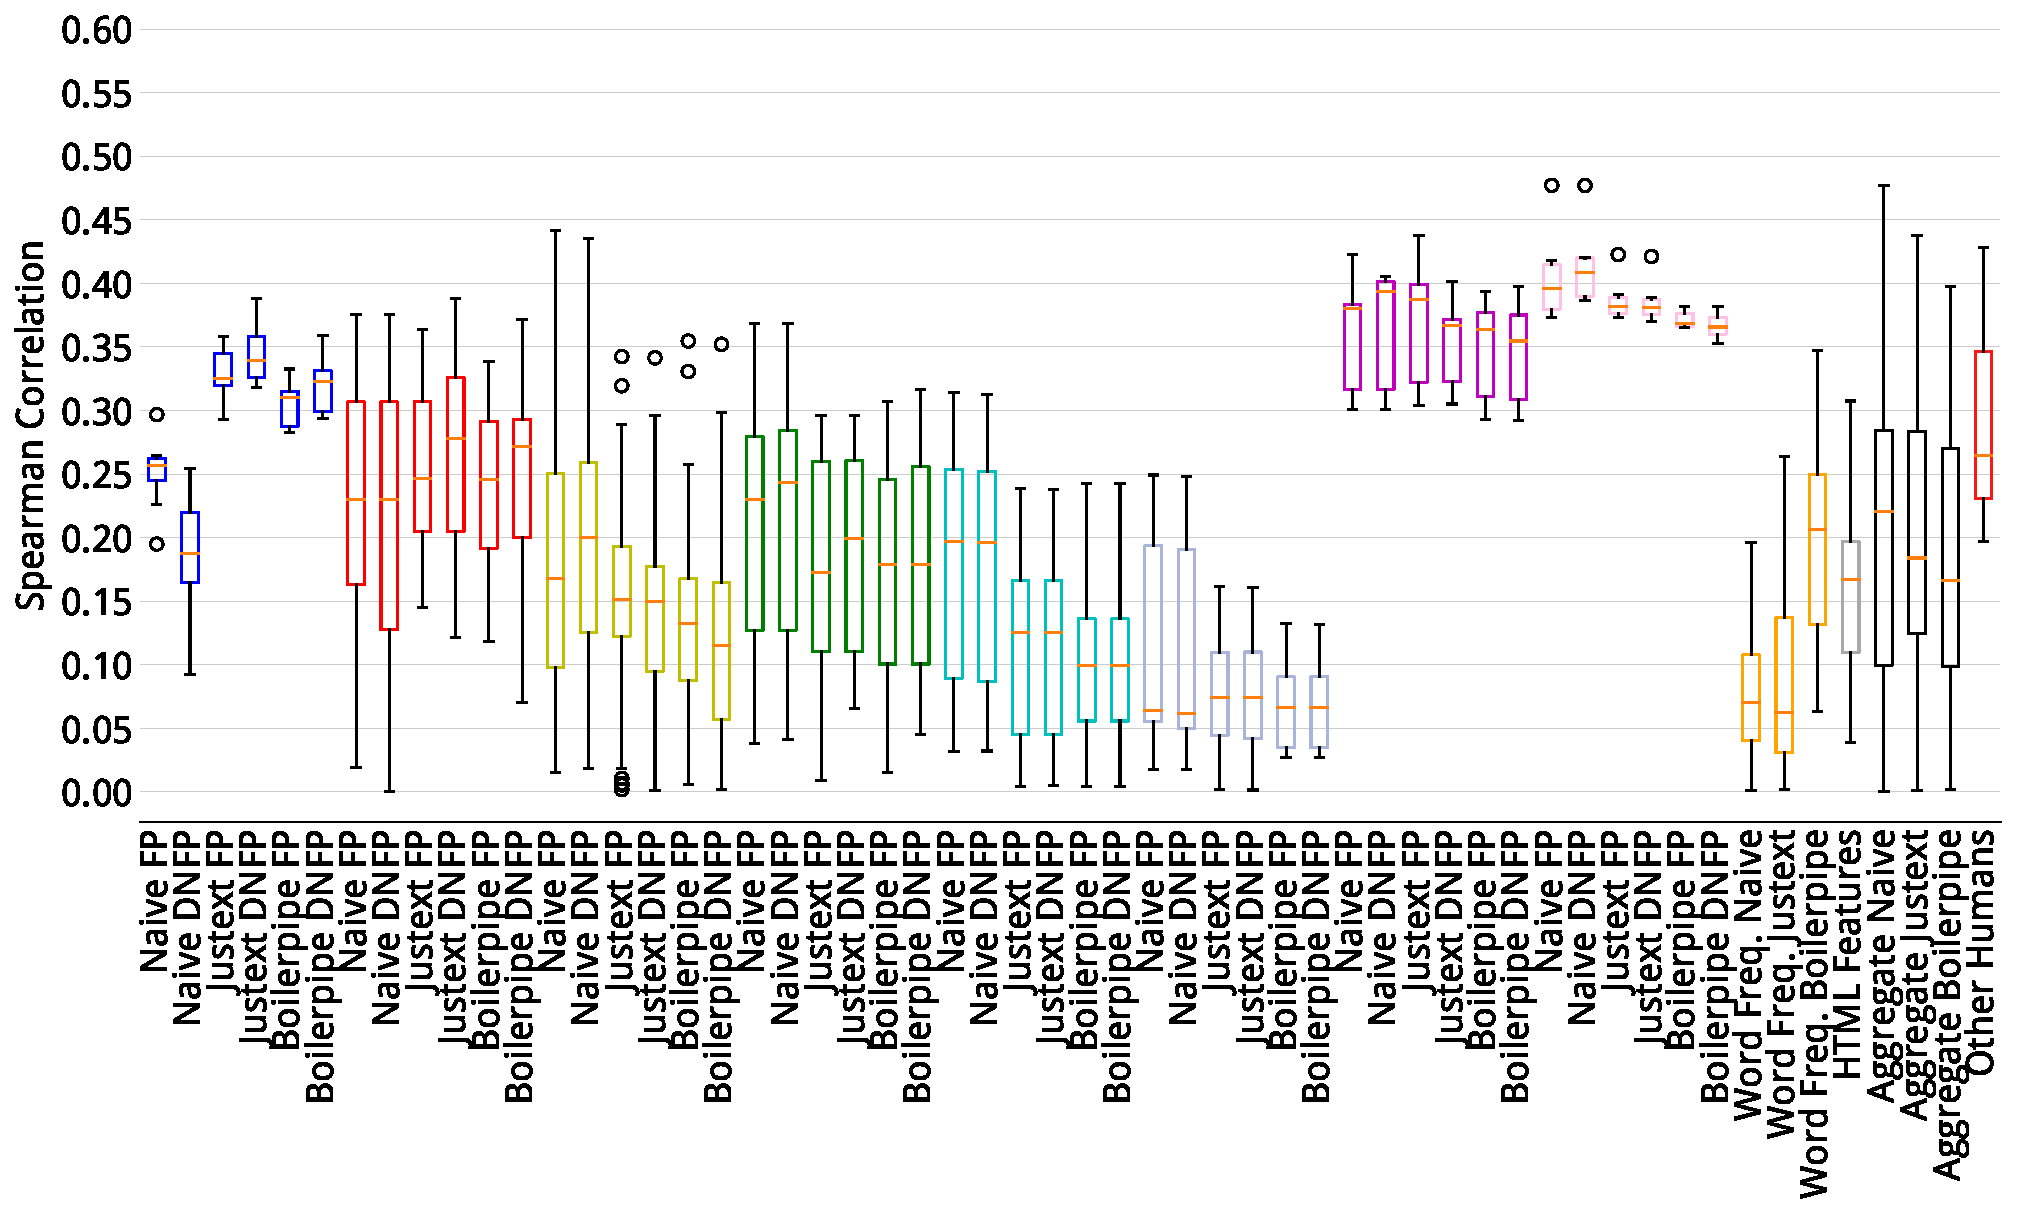
\includegraphics[width=0.90\textwidth]{graphics/box_spearman15_raw_values}
%   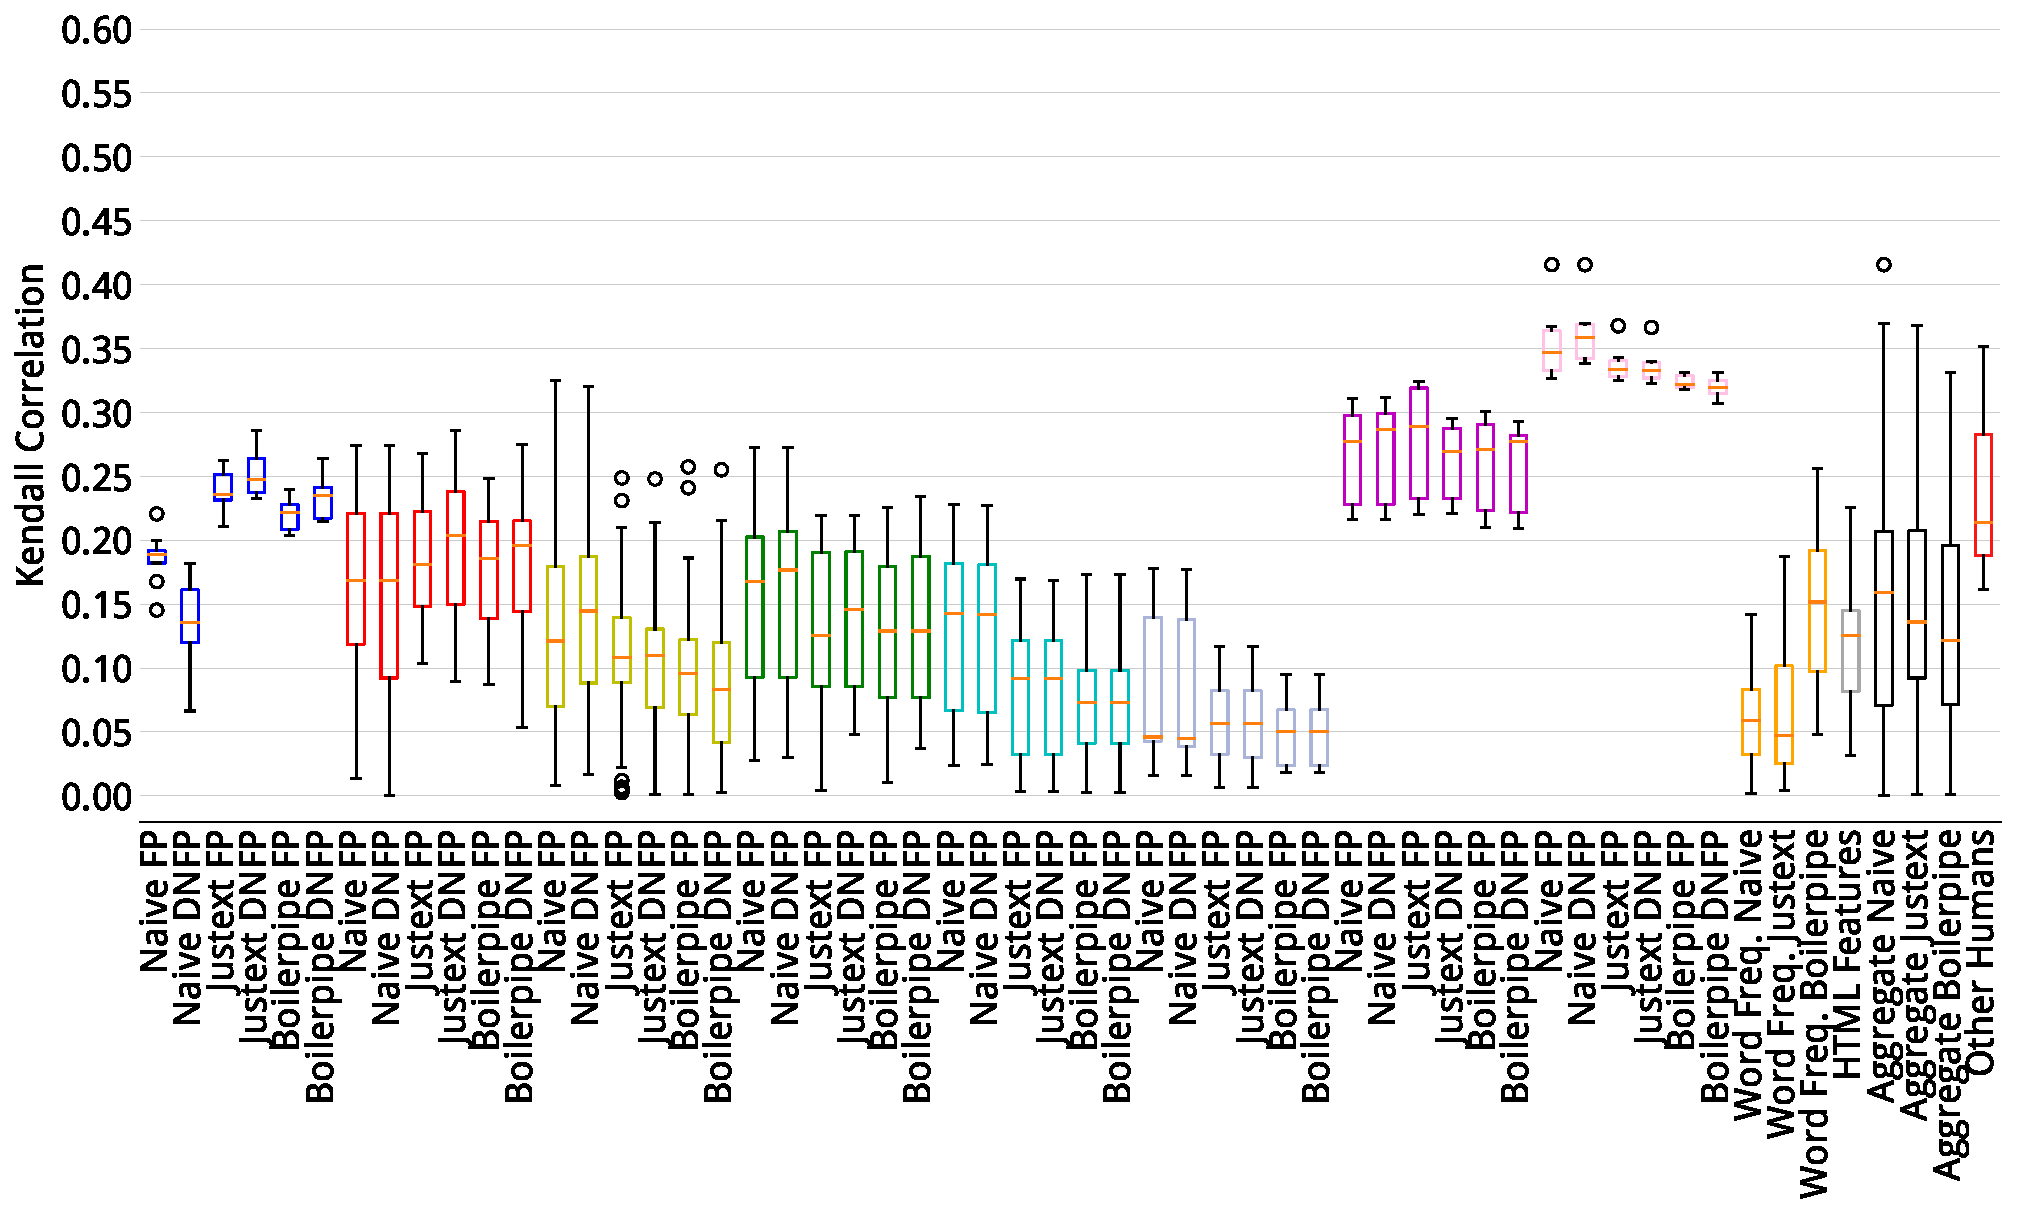
\includegraphics[width=0.90\textwidth]{graphics/box_kendalltau15_raw_values}
%   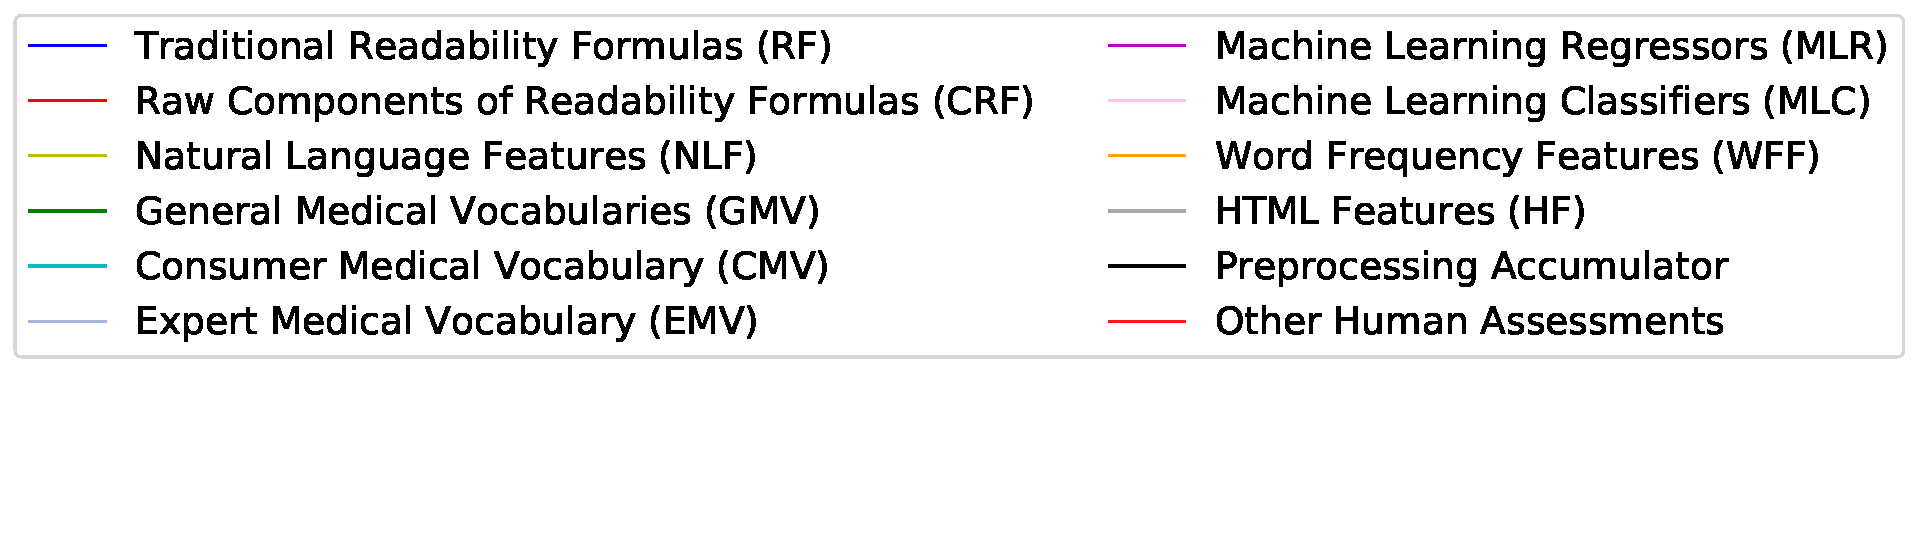
\includegraphics[width=0.65\textwidth]{graphics/legendCorr}
%   \caption{Box plots divided by feature groups. Correlations are calculated using understandability labels from relevant documents assessed in CLEF eHealth 2015}
%   \label{fig:boxplot_corr_docs_2015}
%\end{figure*}

%\begin{figure*}[th!]
%   \centering
%   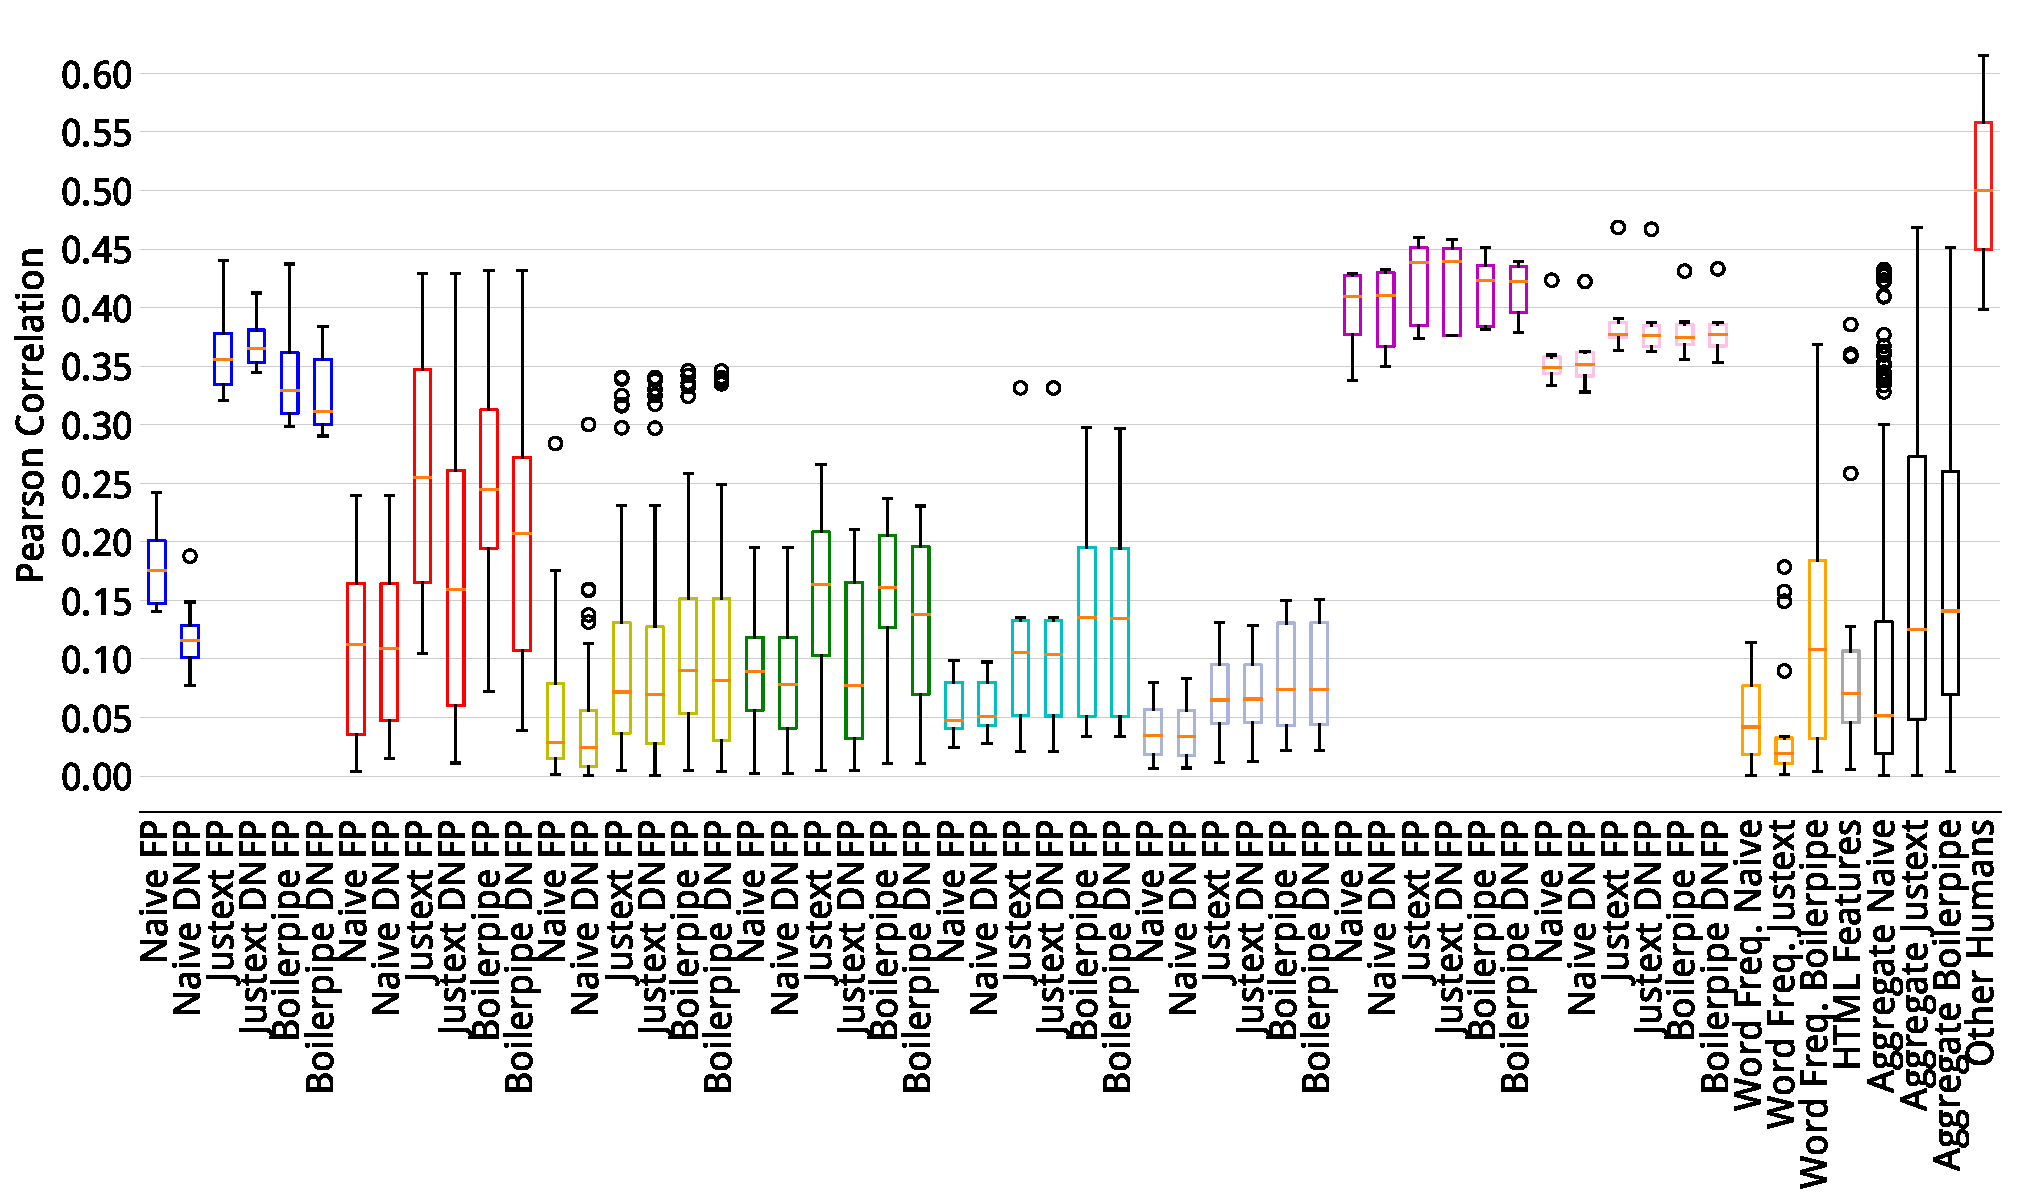
\includegraphics[width=0.90\textwidth]{graphics/box_pearson16_raw_values}
%   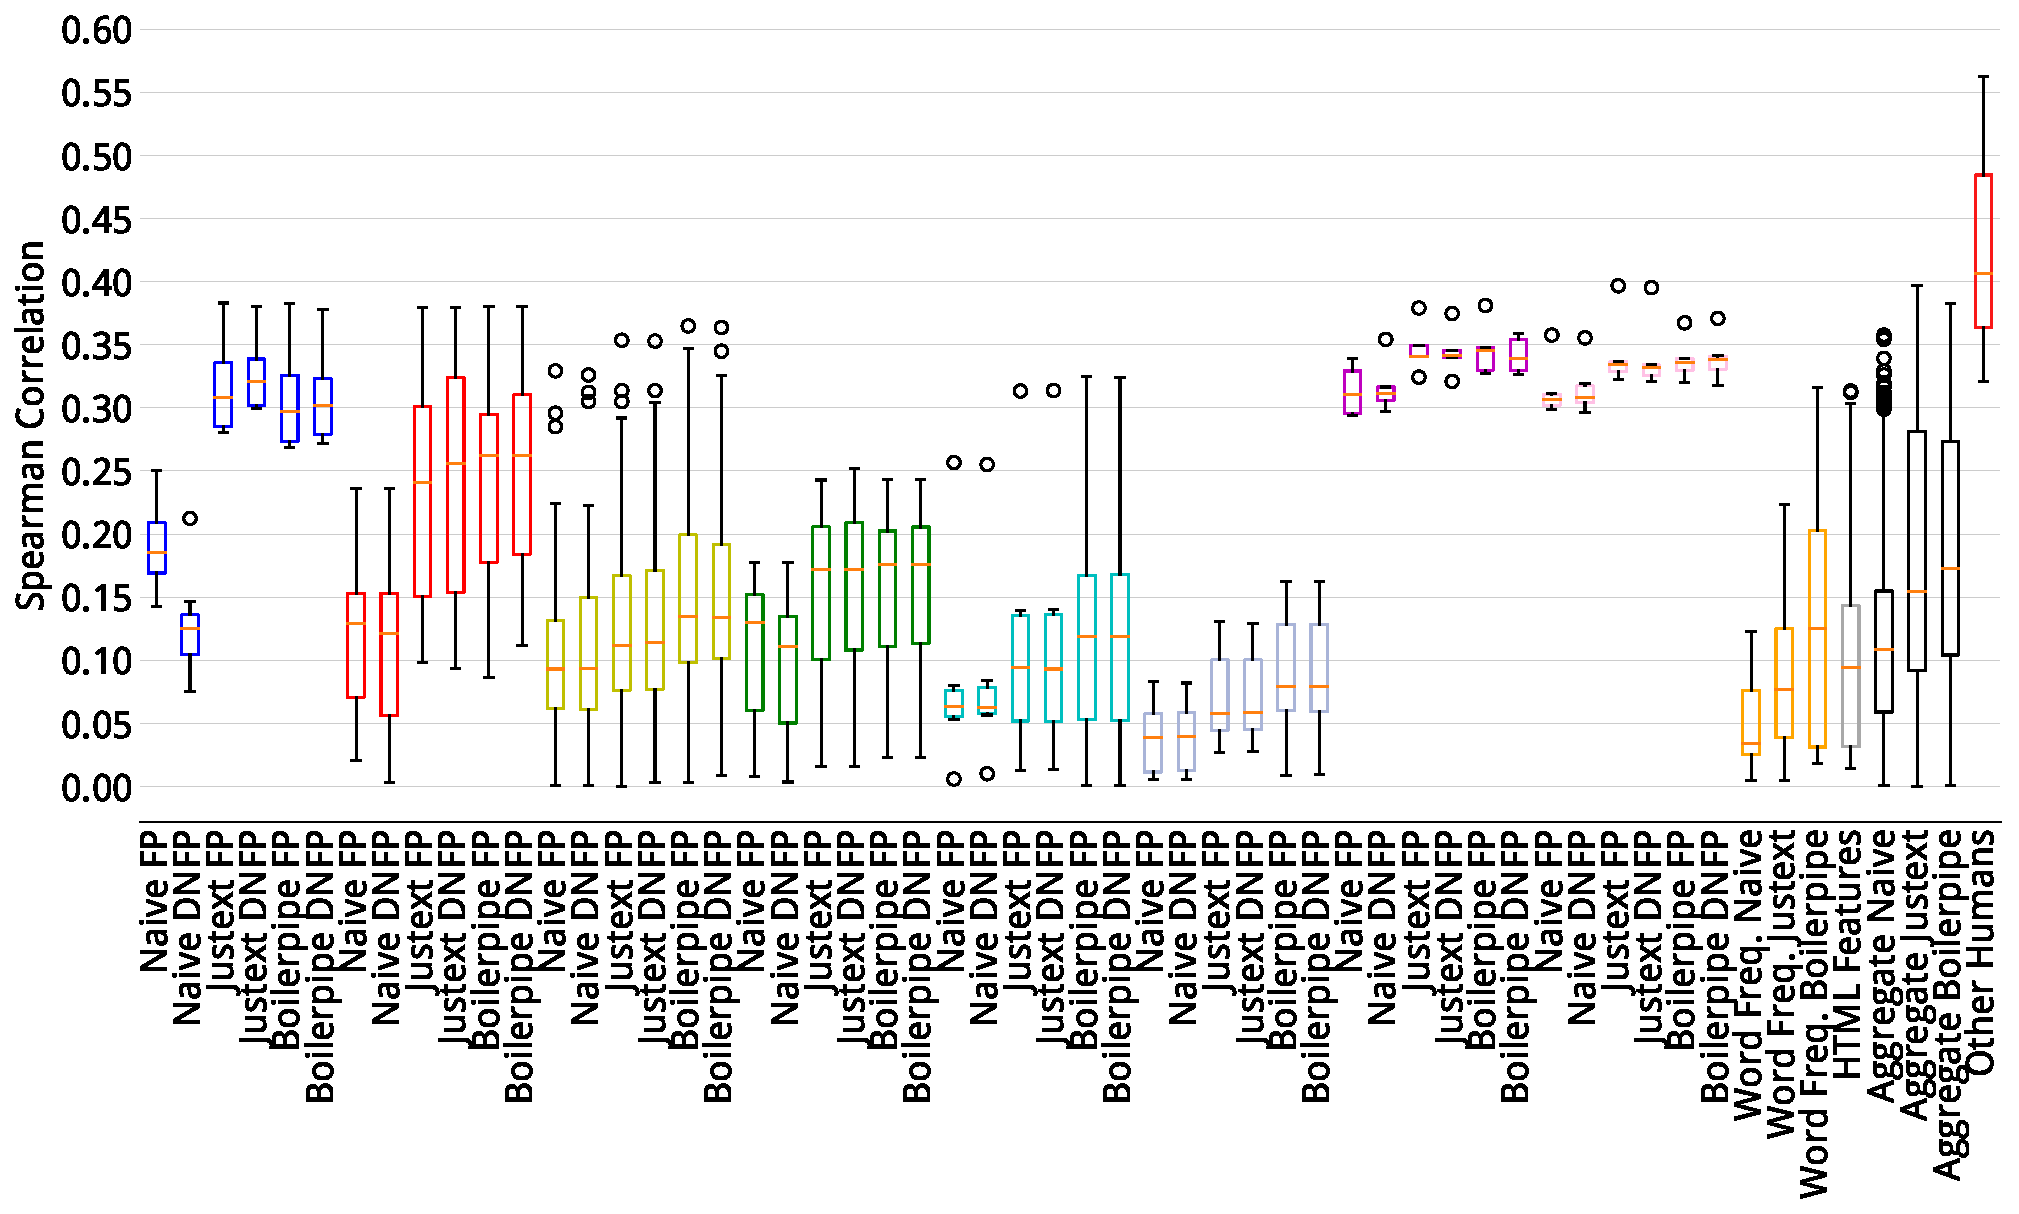
\includegraphics[width=0.90\textwidth]{graphics/box_spearman16_raw_values}
%   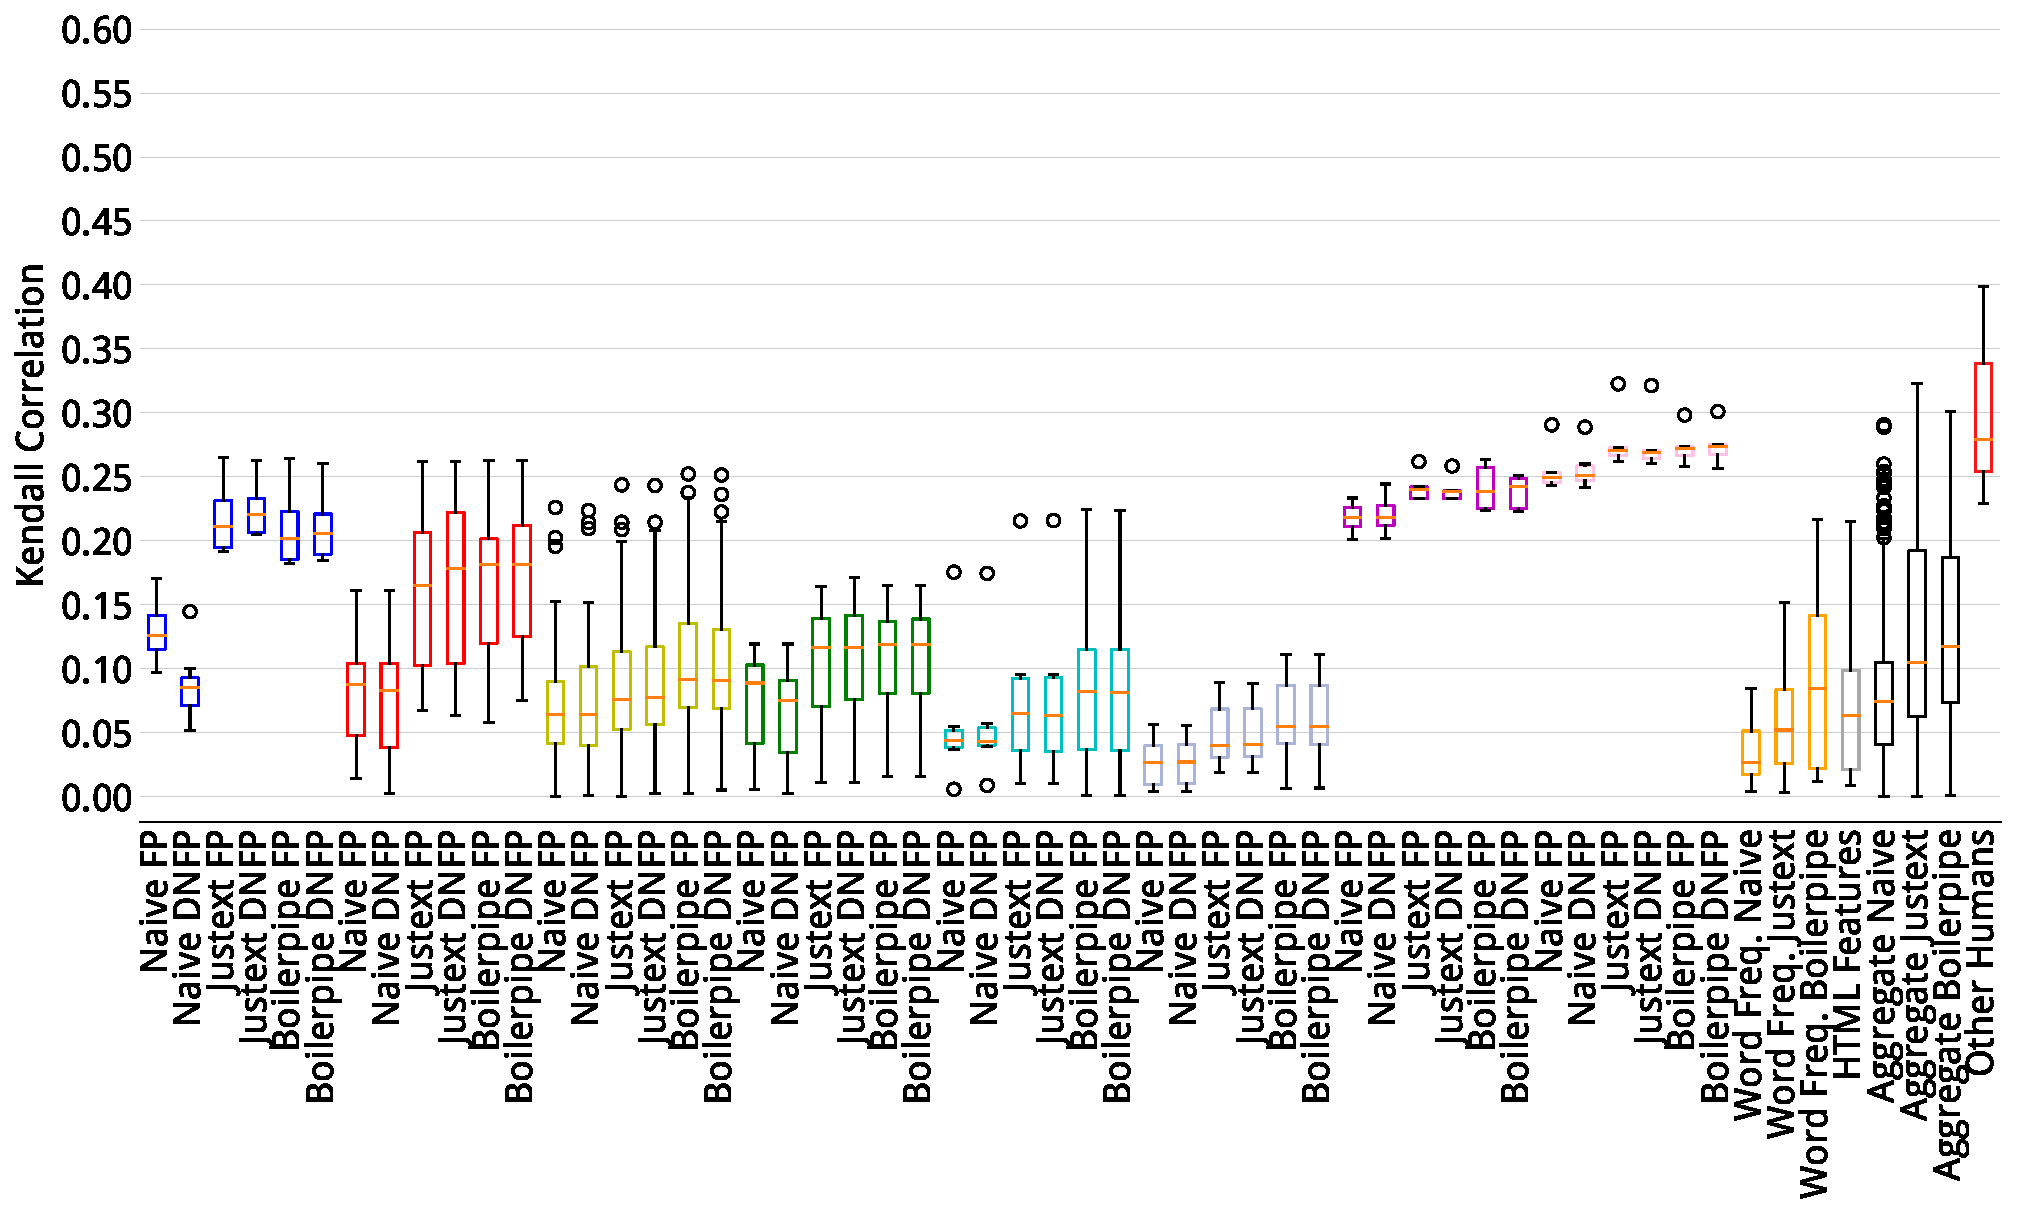
\includegraphics[width=0.90\textwidth]{graphics/box_kendalltau16_raw_values}
%    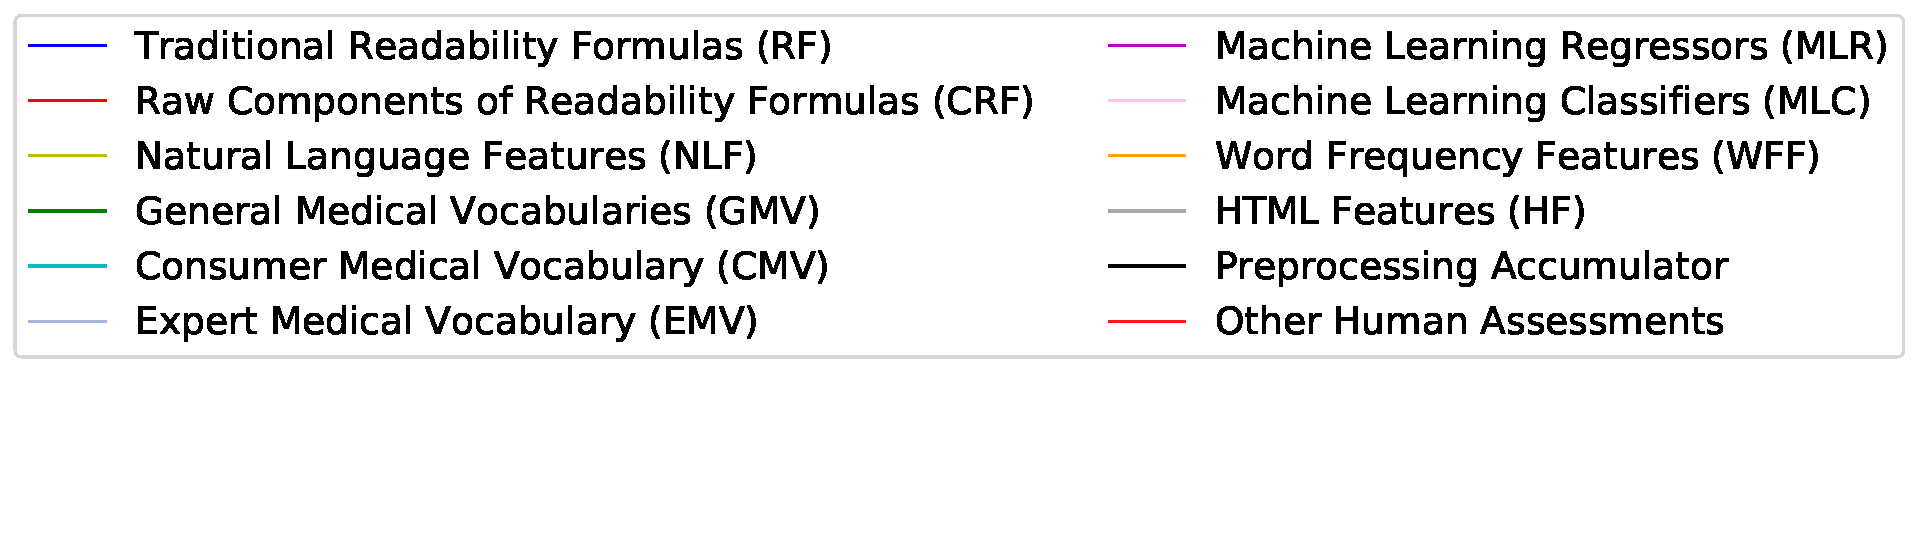
\includegraphics[width=0.65\textwidth]{graphics/legendCorr}
%    \caption{Box plots divided by feature groups. Correlations are calculated using understandability labels from relevant documents assessed in CLEF eHealth 2016}
%   \label{fig:boxplot_corr_docs_2016}
%\end{figure*}

%Figure~\ref{fig:boxplot_corr_docs_2015} shows the correlations for CLEF eHealth 2015 assessments.
%Top part of Figure~\ref{fig:boxplot_corr_docs} shows the Spearman correlation for CLEF eHealth 2015 assessments.

%The choice of preprocessing method had the highest impact on the traditional readability formula group, with the Naive preprocessing clearly underperforming the other preprocessing methods. The choice of the Naive method was also the worst for the word frequency group, but, interestingly, it was a good choice, or at least a competitive one, for all other groups.
%The highest correlations were archived by the regressors and classifiers, independently of the preprocessing method used.

%For this group, all correlation measures point out that the Naive processing yielded the weakest correlation, and Justext was marginally better than Boilerpipe. Comparing the medians, the strategy of DoNotForcePeriod performed better than ForcePeriod. The readability formula group was also the one with higher correlation, with an average correlation equal or higher than the human one.

%Similarly to Figure~\ref{fig:boxplot_corr_docs_2015}, Figure~\ref{fig:boxplot_corr_docs_2016} reports the findings for CLEF eHealth 2016. 
%Similarly the bottom part of Figure~\ref{fig:boxplot_corr_docs} reports the findings for CLEF eHealth 2016. 
%This time, though, the Naive preprocessing method was clearly underperforming for most of the groups analysed, including regressors and classifiers.

%In order to further understand our experiments, we compared the median of each pair of preprocessing strategy showed in Figures~\ref{fig:boxplot_corr_docs_2015} and~\ref{fig:boxplot_corr_docs_2016} and present the results in Table~\ref{tab:comparison_preprocessing}. 

We further analysed the results by performing pairwise comparisons between the median correlations across preprocessing pipelines and heuristics, and reporting the number of times the median correlation of a setting was better than another. These are reported in Table~\ref{tab:comparison_preprocessing}: in brackets we reported the number of comparisons that were statistically significant. 

%In order to further understand our experiments, we present in Table~\ref{tab:comparison_preprocessing} the results of comparing the median of two-by-two for different preprocessing strategies shown in Figure~\ref{fig:boxplot_corr_docs}. We also include the results for Pearson and Kendall correlations.
%For instance, the entry $\mathit{FP < DNFP}$ counts the number of times the median value for \textit{ForcePeriod} was superior to \textit{DoNotForcePeriod} when comparisons with the same HTML cleaning method was used, e.g. \textit{Naive ForcePeriod} versus \textit{Naive DoNotForcePeriod}. From all comparisons, the ones that were statistically significant according to a t-test are shown inside parentheses.

We first examined the comparison between sentence ending heuristics (ForcePeriod (FP) and DoNotForcePeriod (DNFP)). Results showed that the two methods achieved comparable results. Then we examined the comparison between preprocessing pipelines. For these, results for CLEF 2015 were in contrast with those for CLEF 2016. While Naive was marginally better than Boilerpipe and Justext in 2015, it was the worst in the majority of comparisons for 2016. In turn, while Justext was significantly better than Boilerpipe in 2015, they showed balanced results in 2016.
\todo{I think something could be said about ustext and Boilerpipe. Done.}
 

\todo{ARRIVED HERE -- need to merge section 4 and 7.}


%The upper part of Table~\ref{tab:comparison_preprocessing} shows results for the comparisons between ForcePeriod (FP) and DoNotForcePeriod (DNFP). Although the interpretation of readability formulas is drastically affected by this choice of preprocessing, as research indicates~\cite{palotti15}, the correlation results are not.
%The number of times FP reached a higher correlation than DNFP is roughly the same that DNFP was higher than FP.
%The bottom part of Table~\ref{tab:comparison_preprocessing} shows the comparisons made for Naive, Justext and Boilerpipe. Results for CLEF 2015 contrast with 2016, while Naive was sightly better than Boilerpipe and Justext in 2015, it was the worst in almost all 2016 comparisons. Also, the comparisons between Justext and Boilerpipe are exactly the opposite from 2015 to 2016.

%
\begin{table}
\centering    
\caption{Exhaustive Comparison summary using the data from Figures 1.2 and 1.3. Numbers inside parentheses represent the number of tests that yielded p < 0.05 in a two-tailed t-test}
\label{tab:comparison_preprocessing}

\resizebox{1.\textwidth}{!}{
\begin{tabular}{lllllllll}
\toprule
\multirow{2}{*}{\textbf{Comparison}} & \multicolumn{4}{c}{\textbf{CLEF 2015}} & \multicolumn{4}{c}{\textbf{CLEF 2016}}\tabularnewline
\cmidrule(l{2pt}r{2pt}){2-5} \cmidrule(l{2pt}r{2pt}){6-9} 
& \textbf{Pearson} & \textbf{Spearman} & \textbf{Kendall Tau} & \textbf{Total} & \textbf{Pearson} & \textbf{Spearman} & \textbf{Kendall Tau} & \textbf{Total}\tabularnewline
\midrule
FP > DNFP & 8 (0) & 11 (4) & 11 (3) & 30 (7) & 16 (10) & 10 (3) & 11 (4) & 37 (17)\tabularnewline
FP < DNFP & 16 (5) & 12 (5) & 12 (6) & 40 (16) & 8 (0) & 12 (2) & 11 (2) & 31 (4)\tabularnewline
FP == DNFP & 0 & 1 & 1 & 2 & 0 & 2 & 2 & 4\tabularnewline
\midrule
Naive > Justext & 11 (7) & 9 (6) & 9 (5) & 29 (18) & 1 (0) & 0 (0) & 0 (0) & 1 (0)\tabularnewline
Naive < Justext & 6 (4) & 8 (4) & 8 (4) & 22 (12) & 16 (12) & 17 (13) & 17 (13) & 50 (38)\tabularnewline
Naive == Justext & 0 & 0 & 0 & 0 & 0 & 0 & 0 & 0\tabularnewline
Naive > Boilerpipe & 12 (7) & 10 (6) & 10 (5) & 32 (18) & 0 (0) & 0 (0) & 0 (0) & 0 (0)\tabularnewline
Naive < Boilerpipe & 5 (4) & 7 (3) & 7 (3) & 19 (10) & 16 (12) & 17 (13) & 17 (13) & 51 (39)\tabularnewline
Naive == Boilerpipe & 0 & 0 & 0 & 0 & 0 & 0 & 0 & 0\tabularnewline
Justext > Boilerpipe & 10 (7) & 16 (9) & 14 (8) & 40 (24) & 9 (4) & 9 (4) & 4 (2) & 17 (8)\tabularnewline
Justext < Boilerpipe & 7 (2) & 1 (0) & 3 (1) & 11 (3) & 8 (2) & 8 (2) & 13 (2) & 34 (6)\tabularnewline
Boilerpipe == Justext & 0 & 0 & 0 & 0 & 0 & 0 & 0 & 0\tabularnewline
\bottomrule 
\end{tabular}
} % close resizebox
\end{table}

%



\section{Integrating Understandability into Retrieval}
\label{sec:experiments}

Next, we investigate how understandability estimations could be used and integrated into retrieval methods to increase the quality of search result. To this aim, we first investigated re-ranking search results from an initial run purely based on understandability estimations. 

Specifically, we considered three retrieval methods of differing quality for the initial retrieval. These included the best two runs submitted to each CLEF task (2015 and 2016), and a plain BM25 baseline (default Terrier parameters: $b=0.75$ and $k1=1.2$). As understandability estimators we used  eXtreme Gradient Boosting (XGB)\footnote{For assessed documents, we used 10-fold cross validation, so that we trained XGB on 90\% of the data, and used its predictions for the remaining 10\%. For unassessed documents, we trained XGB on all assessed data, and applied this model to generate predictions.} regressor, as well as SMOG for CLEF 2015 and Dale-Chall for CLEF 2016. These were the best performing approaches from Section~\ref{sec:beyond_readability}.

If all the search results from a run were considered, then such a re-ranking method may place at early ranks Web pages highly likely to be understandable, but possibly less likely to be topically relevant. To balance relevance and understandability, we only re-ranked the first $k$ documents. We explored $k = 15, 20, 50$. Because evaluation was performed with respect to the first $n=10$ rank positions, the setting $k=15$ provided a conservative re-ranking of search results; while, $k=50$ provided a more speculative re-ranking approach. Results are presented in Section~\ref{results:reranking}.

As an alternative to the previous two-step ranking strategy for combining topical relevance and understandability, we explored the fusion of two search results lists separately obtained for relevance and understandability. For this, we used the Reciprocal Rank Fusion (RRF) method~\cite{cormack09}, which has proven effective for combining two lists of search results based on their documents \textit{ranks}, rather than scores. This approach was selected above score-based fusion methods because of the different scoring strategies and distributions employed when scoring for relevance compared to for understandability. For topical relevance, we used, separately, the three methods used for re-ranking (\todo{XXXbest runsXXX} for CLEF2015, GUIR and ECNU for CLEF 2016, and BM25 for both collections). For understandability, we used, separately, the estimations from SMOG/Dale Chall and XGB. Also for this approach we studied limiting the ranking of results to be considered by the methods across the cut-offs $k=15, 20, 50$. Results are presented in Section~\ref{results:fusion}.

Finally, we considered a third alternative to combine topical relevance and understandability: using learning to rank with features derived from the retrieval method and the understandability estimators.
In this experiment, we explored different label attribution and feature sets, keeping the same learning to rank algorithm, again XGB. We first experiment with settings made to optimise only relevance (we consider different Information Retrieval models (BM25, L as feature

\todo{need more details: In the LTR we need to mention the combination of labels to make up the final document label which will be used by the method. Also, we need to say which method we used (pairwise tree boosting) and which are the features for each run.... Note, we only performed learning to rank on the BM25 baseline, because we do not have access to the retrieval features used in the CLEF submissions.}. Results are presented in Section~\ref{results:ltr}.

\begin{table*}[ht!]
\caption{Results obtained by integrating understandability estimations within
retrieval methods on CLEF 2016. Baseline runs are reported at table
indices 1-3. Re-ranking experiments are reported at indices 4-21.
Fusion experiments are reported at indices 22-30. Learning to rank
experiments are reported at indices 31-35. All measures were calculated
up to rank $n=10$. }
%\vspace{-0.2cm}
 \label{tab:experiments} 
\resizebox{1.00\textwidth}{!}{ %
\begin{tabular}{cclllllllllllll}
\toprule 
    \multirow{2}{*}{Index }  & \multirow{2}{*}{Rerank }  & \multirow{2}{*}{Run }  & \multicolumn{4}{l}{Official CLEF 2016 Metrics} & \multicolumn{8}{l}{New Metrics to Evaluate Underst. in Retrieval - Sec.~\ref{sec:data}}\tabularnewline
\cmidrule(l{2pt}r{2pt}){4-7} \cmidrule(l{2pt}r{2pt}){8-15}  &  &  & $RBP$  & RBP Res.  & uRBP  & uRBP Res.  & $RBP_{u}$  & $RBP_{u}$ Res. & $HRBP$  & HRBP Res. & Unj  & $RBP_{r}^{*}$  & $RBP_{u}^{*}$  & $HRBP^{*}$\tabularnewline
\midrule 
1  & \multirow{3}{*}{No Rerank}  & GUIR~\cite{soldaini16} (Best Run)  & \textbf{28.11}  & 7.65  & \textbf{18.12}  & 7.19  & \textbf{45.69}  & 8.86 & \textbf{25.61}  & 6.50 & 0.01  & \textbf{28.29}  & \textbf{46.03}  & \textbf{25.79} \tabularnewline
2  &  & ECNU~\cite{song16} (Runner Up)  & 27.70  & 7.37  & 17.55  & \textbf{7.34}  & 43.89$^{\diamond}$  & 8.66 & 25.35  & 6.26 & 0.01  & 27.77  & 44.18$^{\diamond}$  & 25.48 \tabularnewline
3  &  & Plain BM25 Baseline  & 25.28$^{\diamond}$  & \textbf{8.24}  & 16.05$^{\diamond}$  & 6.94  & 42.08$^{\diamond}$  & \textbf{10.97} & 22.97$^{\diamond}$  & \textbf{7.19} & \textbf{0.06}  & {26.01}$^{\diamond}$  & {43.89}$^{\diamond}$  & {23.93}$^{\diamond}$ \tabularnewline
\midrule 
4  & \multirow{3}{*}{\makecell{Dale-Chall Top 15}}  & Based on GUIR  & 24.70$^{\dagger\diamond}$  & 8.70  & 16.83$^{\dagger\diamond}$  & 7.27  & 49.10$^{\dagger\diamond}$  & 10.62 & 24.94  & 7.50 & 0.03  & 25.24$^{\dagger\diamond}$  & 50.33$^{\dagger\diamond}$  & 25.54 \tabularnewline
5  &  & Based on ECNU  & 24.78$^{\dagger\diamond}$  & 7.83  & 16.64$^{\diamond}$  & 7.16  & 48.88$^{\dagger\diamond}$  & 9.71 & 24.80  & 6.50 & 0.02  & 25.12$^{\dagger\diamond}$  & 49.64$^{\dagger\diamond}$  & 25.21 \tabularnewline
6  &  & Based on BM25  & 23.22$^{\dagger\diamond}$  & 8.78  & 15.85 $^{\diamond}$  & 6.94  & 47.09$^{\dagger\diamond}$  & 11.83 & 24.01  & 7.42 & 0.07  & 24.04$^{\dagger\diamond}$  & 48.60$^{\dagger\diamond}$  & 24.82 \tabularnewline
\hdashline 7  & \multirow{3}{*}{\makecell{Dale-Chall Top 20}}  & Based on GUIR  & 22.19$^{\dagger\diamond}$  & 9.37  & 15.36$^{\dagger\diamond}$  & 6.98  & 48.71$^{\dagger\diamond}$  & 12.30 & 23.21$^{\dagger\diamond}$  & 8.12 & 0.06  & 23.26$^{\dagger\diamond}$  & 51.39$^{\dagger\diamond}$  & 24.45$^{\dagger\diamond}$\tabularnewline
8  &  & Based on ECNU  & 23.01$^{\dagger\diamond}$  & 8.93  & 15.70$^{\dagger\diamond}$  & 6.91  & 48.99$^{\dagger\diamond}$  & 11.69 & 23.73$^{\dagger\diamond}$  & 7.80 & 0.05  & 23.84$^{\dagger\diamond}$  & 51.00$^{\dagger\diamond}$  & 24.66\tabularnewline
9  &  & Based on BM25  & 21.58$^{\dagger\diamond}$  & 9.51  & 14.83$^{\dagger\diamond}$  & 7.02  & 46.99$^{\dagger}$  & 13.00 & 22.89$^{\diamond}$  & 8.06 & 0.09  & 22.93$^{\dagger\diamond}$  & 49.55$^{\dagger\diamond}$  & 24.26\tabularnewline
\hdashline 10  & \multirow{3}{*}{\makecell{Dale-Chall Top 50}}  & Based on GUIR  & 16.18$^{\dagger\diamond}$  & 15.24  & 11.56$^{\dagger\diamond}$  & 6.80  & 41.79$^{\dagger\diamond}$  & 24.49 & 18.10$^{\dagger\diamond}$  & 14.42 & 0.22  & 20.90$^{\dagger\diamond}$  & 53.28$^{\dagger\diamond}$  & 23.27$^{\dagger\diamond}$ \tabularnewline
11  &  & Based on ECNU  & 16.88$^{\dagger\diamond}$  & 17.37  & 11.78$^{\dagger\diamond}$  & \textbf{7.30}  & 40.76$^{\dagger\diamond}$  & 23.77 & 18.30$^{\dagger\diamond}$  & \textbf{15.57} & \textbf{0.24}  & 21.34$^{\dagger\diamond}$  & 52.07$^{\dagger\diamond}$  & 23.33$^{\dagger\diamond}$ \tabularnewline
12  &  & Based on BM25  & 15.06$^{\dagger\diamond}$  & 15.35$^{\dagger\diamond}$  & 10.55  & 6.62  & 40.03 $^{\diamond}$  & 23.88 & 16.55$^{\dagger\diamond}$  & 13.83 & \textbf{0.24}  & 19.42$^{\dagger\diamond}$  & 51.69$^{\dagger\diamond}$  & 21.59$^{\dagger\diamond}$ \tabularnewline
\hdashline 13  & \multirow{3}{*}{\makecell{XGB Top 15}}  & Based on GUIR  & \textbf{25.16}$^{\dagger\diamond}$  & 8.09  & \textbf{17.27}$^{\dagger\diamond}$  & 7.12  & \textbf{50.96}$^{\dagger\diamond}$  & 10.11 & \textbf{25.16}  & 6.89 & 0.02  & \textbf{25.61}$^{\dagger\diamond}$  & 52.00$^{\dagger\diamond}$  & \textbf{25.68}\tabularnewline
14  &  & Based on ECNU  & 24.18$^{\dagger\diamond}$  & 7.69  & 16.54 $^{\diamond}$  & 7.09  & 50.00$^{\dagger\diamond}$  & 9.91 & 24.56  & 6.65 & 0.02  & 24.56$^{\dagger\diamond}$  & 50.74$^{\dagger\diamond}$  & 25.01\tabularnewline
15  &  & Based on BM25  & 22.33$^{\dagger\diamond}$  & 8.14  & 15.46  & 6.76  & 47.90$^{\dagger\diamond}$  & 12.13 & 22.89$^{\diamond}$  & 7.25 & 0.07  & 23.11$^{\dagger\diamond}$  & 49.43$^{\dagger\diamond}$  & 23.69$^{\diamond}$\tabularnewline
\hdashline 16  & \multirow{3}{*}{\makecell{XGB Top 20}}  & Based on GUIR  & 22.38$^{\dagger\diamond}$  & 9.49  & 15.61$^{\dagger\diamond}$  & 7.05  & 50.45$^{\dagger\diamond}$  & 12.08 & 23.30$^{\dagger\diamond}$  & 8.16 & 0.05  & 23.62$^{\dagger\diamond}$  & 52.98$^{\dagger\diamond}$  & 24.68\tabularnewline
17  &  & Based on ECNU  & 22.95$^{\dagger\diamond}$  & 8.82  & 15.95$^{\dagger\diamond}$  & 7.02  & 50.42$^{\dagger\diamond}$  & 11.70 & 23.97$^{\diamond}$  & 7.56 & 0.04  & 23.68$^{\dagger\diamond}$  & 52.15$^{\dagger\diamond}$  & 24.73\tabularnewline
18  &  & Based on BM25  & 20.65$^{\dagger\diamond}$  & 9.42  & 14.46$^{\dagger\diamond}$  & 6.84  & 47.74$^{\dagger\diamond}$  & 13.56 & 21.93$^{\diamond}$  & 8.34 & 0.09  & 21.98$^{\dagger\diamond}$  & 50.28$^{\dagger\diamond}$  & 23.27$^{\diamond}$\tabularnewline
\hdashline 19  & \multirow{3}{*}{\makecell{XGB Top 50}}  & Based on GUIR  & 16.65$^{\dagger\diamond}$  & 15.73  & 12.39$^{\dagger\diamond}$  & 6.84  & 43.49$^{\dagger\diamond}$  & 23.63 & 18.70$^{\dagger\diamond}$  & 13.74 & 0.22  & 21.13$^{\dagger\diamond}$  & \textbf{55.07}$^{\dagger\diamond}$  & 23.58$^{\dagger\diamond}$\tabularnewline
20  &  & Based on ECNU  & 16.19$^{\dagger\diamond}$  & \textbf{17.01}  & 11.82$^{\dagger\diamond}$  & 7.27  & 43.05$^{\diamond}$  & \textbf{24.75} & 18.27$^{\dagger\diamond}$  & 14.41 & \textbf{0.24}  & 20.16$^{\dagger\diamond}$  & 54.70$^{\dagger\diamond}$  & 22.96$^{\dagger\diamond}$\tabularnewline
21  &  & Based on BM25  & 15.43$^{\dagger\diamond}$  & 15.37  & 11.33$^{\dagger\diamond}$  & 6.48  & 41.93$^{\diamond}$  & 23.65 & 17.43$^{\dagger\diamond}$  & 13.40 & 0.26  & 19.58$^{\dagger\diamond}$  & 54.04$^{\dagger\diamond}$  & 22.17$^{\dagger\diamond}$\tabularnewline
\midrule 
22  & \multirow{3}{*}{\makecell{RRF (XGB \& Orig.) Top 15} }  & Based on GUIR  & \textbf{27.23}$^{\dagger\diamond}$  & 7.76  & \textbf{18.31}  & \textbf{7.23}  & 49.69$^{\dagger\diamond}$  & 9.18 & 26.49$^{\dagger\diamond}$  & 6.62 & 0.01  & \textbf{27.46}$^{\dagger\diamond}$  & 50.07$^{\dagger\diamond}$  & \textbf{26.69}$^{\dagger\diamond}$\tabularnewline
23  &  & Based on ECNU  & 26.60$^{\dagger\diamond}$  & 7.41  & 17.81  & 7.19  & 48.67$^{\dagger\diamond}$  & 8.80 & 26.02  & 6.09 & 0.01  & 26.76$^{\dagger\diamond}$  & 49.10$^{\dagger\diamond}$  & 26.27$^{\dagger}$ \tabularnewline
24  &  & Based on BM25  & 24.57$^{\diamond}$  & 8.15  & 16.51$^{\diamond}$  & 6.91  & 46.76$^{\dagger}$  & 11.23 & 24.16$^{\dagger}$  & 7.20 & 0.06  & 25.32$^{\diamond}$  & 48.52$^{\dagger\diamond}$  & 25.08$^{\dagger}$ \tabularnewline
\hdashline 25  & \multirow{3}{*}{\makecell{RRF (XGB \& Orig.) Top 20}}  & Based on GUIR  & 26.21$^{\dagger\diamond}$  & 7.96  & 17.73  & 7.19  & 50.29$^{\dagger\diamond}$  & 9.58 & 25.89  & 6.73 & 0.03  & 26.53$^{\dagger\diamond}$  & 50.98$^{\dagger\diamond}$  & 26.25\tabularnewline
26  &  & Based on ECNU  & 26.15$^{\dagger\diamond}$  & 7.64  & 17.69  & 7.09  & 49.70$^{\dagger\diamond}$  & 9.28 & \textbf{26.07 } & 6.39 & 0.02  & 26.38$^{\dagger\diamond}$  & 50.32$^{\dagger\diamond}$  & 26.35\tabularnewline
27  &  & Based on BM25  & 24.04$^{\dagger\diamond}$  & 8.24  & 16.32$^{\diamond}$  & 6.87  & 47.69$^{\dagger\diamond}$  & 11.40 & 24.08$^{\dagger\diamond}$  & 7.35 & 0.06  & 24.82$^{\dagger\diamond}$  & 49.52$^{\dagger\diamond}$  & 25.01$^{\dagger}$ \tabularnewline
\hdashline 28  & \multirow{3}{*}{\makecell{RRF (XGB \& Orig.) Top 50}}  & Based on GUIR  & 24.09$^{\dagger\diamond}$  & \textbf{9.44}  & 16.85$^{\dagger\diamond}$  & 7.02  & 50.55$^{\dagger\diamond}$  & 11.76 & 24.76  & \textbf{8.01} & 0.07  & 25.08$^{\dagger\diamond}$  & \textbf{52.84}$^{\dagger\diamond}$  & 25.84\tabularnewline
29  &  & Based on ECNU  & 24.17$^{\dagger\diamond}$  & 8.67  & 16.75$^{\diamond}$  & 7.12  & \textbf{50.63}$^{\dagger\diamond}$  & 11.66 & 25.00  & 7.61 & 0.07  & 24.90$^{\dagger\diamond}$  & 52.50$^{\dagger\diamond}$  & 25.84 \tabularnewline
30  &  & Based on BM25  & 22.28$^{\dagger\diamond}$  & 8.87 & 15.50  & 6.76  & 48.79$^{\dagger\diamond}$  & \textbf{12.90} & 23.13$^{\dagger\diamond}$  & 7.82 & \textbf{0.10 } & 23.46$^{\dagger\diamond}$  & 51.89$^{\dagger\diamond}$  & 24.57\tabularnewline
\midrule 
31  & \multirow{5}{*}{XGB LeToR}  & Combo 1 on BM25  & 20.42$^{\dagger\diamond}$  & 17.61  & 13.00$^{\dagger\diamond}$  & 7.41  & 32.17$^{\dagger\diamond}$  & 24.61 & 18.39$^{\dagger\diamond}$  & 14.41 & 0.28  & 25.25$^{\diamond}$  & 43.19$^{\diamond}$  & 23.83$^{\diamond}$\tabularnewline
32  &  & Combo 2 on BM25  & 24.98$^{\dagger\diamond}$  & 19.83  & 15.30$^{\dagger\diamond}$  & 8.09  & 35.09$^{\dagger\diamond}$  & 25.14 & 22.26$^{\diamond}$  & 17.50 & 0.24  & 30.41  & 46.09  & 28.28$^{\dagger\diamond}$ \tabularnewline
33  &  & Combo 3 on BM25  & 26.35$^{\dagger}$  & \textbf{20.48}  & 15.88$^{\dagger\diamond}$  & 8.16  & 34.73$^{\dagger\diamond}$  & 24.69 & 21.81$^{\dagger}$  & 17.41 & 0.22  & 32.25$^{\diamond}$  & 45.44  & 28.22$^{\dagger\diamond}$\tabularnewline
34  &  & Combo 4 on BM25  & 16.16$^{\dagger\diamond}$  & 19.48  & 10.76$^{\dagger\diamond}$  & 7.27  & \textbf{36.75}$^{\dagger\diamond}$  & \textbf{28.51} & 16.77$^{\dagger\diamond}$  & \textbf{17.80} & \textbf{0.29 } & 22.20$^{\dagger\diamond}$  & \textbf{50.06}$^{\dagger\diamond}$  & 23.32$^{\diamond}$\tabularnewline
35  &  & Combo 5 on BM25  & \textbf{26.76}$^{\diamond}$  & \textbf{20.48}  & \textbf{16.19}$^{\diamond}$  & \textbf{8.34}  & 35.26$^{\dagger\diamond}$  & 24.13 & \textbf{22.96}  & 17.59 & 0.22  & \textbf{32.60}$^{\dagger}$  & 45.87  & \textbf{29.20}$^{\dagger\diamond}$\tabularnewline
\bottomrule
\end{tabular}
} % end of resizebox
\end{table*}



\vspace{-10pt}
\section{Evaluation of Understandability Retrieval}
\label{sec:results}

We report the results obtained when experimenting with the retrieval methods described above in Table~\ref{tab:experiments}. We report only the results for CLEF 2016 (thus we only report Dale Chall) for brevity; those on CLEF 2015 exhibited similar trends and are included in the online appendix. The effectiveness of the top two submission to CLEF 2016 and the BM25 baseline are reported at indices 1-3 of the table. Statistical significant differences compared to the best participating run, GUIR, are reported with $\diamond$; differences between the original run (indices 1-3) and its modification are reported with $\dagger$ (paired, two-tail t-test, $p<0.05$). Note that the baseline BM25 is significantly worse than GUIR across all measures. \todo{JP: actually note that the dagger IS NOT a comparison with ECNU, rather it is comparing a modified run with the original version} 

%We start our experiments by showing at the top of Table~\ref{tab:experiments} (indices 1-3) the performance of the top 3 systems in CLEF eHealth 2016 together with a straightforward BM25 baseline run made with Terrier toolkit. Our further experiments will use not only these runs as a comparison base, but modify these runs when necessary.

\subsection{Re-ranking}
\label{results:reranking}

Indices 4-6 of Table~\ref{tab:experiments} report on our experiments re-ranking documents from runs listed at indices 1-3, up to rank 20, according to their Dale-Chall index.
We find that the topical relevance of the re-ranked runs, represented by $NDCG_r$ significantly decreases when compared to their original runs. For example, the $NDCG_r$ of the re-ranked Dale-Chall version of BM25 decreased from 22.02 to 18.53. However, the re-ranked results were significantly more understandable, as reported by their $NDCG_u$. 
Note a limitation of RBP or uRBP metrics to reveal such trend, as both relevance and understandability are tied together.
% As the number of unassessed documents increases ($Una@10$)

Next, we swap the Dale-Chall Index by XGB regressor trained using all features of Table~\ref{tab:doc_features}\footnote{Experiments with various Machine Learning methods and feature selection schemes were performed as well and are available in the online appendix. The results of other methods are similar.}. % When using the set of top 10 features for each group from Table~\ref{tab:top_corr_metrics} results are always better than using an automatic method such as Chi Square to select 10 features to use.}.
%While the higher correlation of Dale-Chall was XXX (as reported in table Y), correlations using XGB reached YYY, the closest method to the human agreement in this task.
We experiment with re-ranking at cut-off 15 (more more conservative method), 20 and 50 (a more heterodox method). 
A similar understandability-relevance trade-off is seen when using a machine learning regressor in place of the Dale-Chall index.
Note that, for the same cut-off value\footnote{We shown here only Dale-Chall cut-off of 20 for brevity.}, the machine learning method consistently yields more understandable results (higher $NDCG_u$). 

\subsection{Rank Fusion}
\label{results:fusion}

Next, from the index 16 to 24, we report the results of our approach to automatically combine topical relevance and understandability through rank fusion.
Once more, allowing re-ranks at higher cut-offs result in larger gains in terms of understandability, but in small losses in terms of topical relevance.
However, the combination of understandability and relevance, $H_ru$, is more stable now than for the previous re-rank methods. 
For example, compare the $H_{ru}^*$ of 13 (21.97) and 22 (24.34) with the original run at index 1 (24.77).

\subsection{Learning to Rank}
\label{results:ltr}

Last, we evaluate our experiments with learning to rank. 


Our final batch of experiments, indices 32-34, are based on learning-to-rank. We decided to use the pairwise implementation of the gradient boosting approach from the XGBoost framework~\cite{chen16} due to its recent good results in many machine learning tasks \todo{actually, I should use XGBoost method instead of LR}. Evaluating other learning to rank methods and frameworks are left as future work.
We evaluated three different settings based on the plain BM25 run shown in index 4, each one with a different combination of feature set and relevance labels:
\begin{itemize}
    \item Index 32: we used as relevance labels only the topical labels and as feature set the score of different information retrieval models (BM25, Dirichlet LM and PL2). This represents the typical use of learning to rank aiming to optimize only the topical relevance results. Unfortunately that was not the case and not even the $P_r@10*$ was improved.
    \item Index 33: we used as relevance labels the linear combination of topical relevance and understandability. Additionally to the IR features, we used the 10 features correspondent to the best features according to Kendall tau in Table~\ref{tab:top_corr_metrics}. Results show that this resulted in higher $F_{ur}*$ when compared to its correspondent approaches (indices 4, 8, 12, 16, 19, 23, 27 and 31) due to a high increase in $P_r@10*$, which reveals understandability features improving topicability.
    \item Index 34: On top of our previous run, we included here all features shown in Table~\ref{tab:doc_features}. Note that despite the very high number of unassessed documents, this run shows improvements even in $P_r@10$ obtaining the same results as the third best run in the campaign (ECNU). In its turn, the $P_{r}*$ which ignores the unassessed documents is 8.4\% higher than the best system, while $F_{ru}*$ is 5.2\% higher.
\end{itemize}







\section{Conclusion}
\label{sec:conclusion_doc_analysis}

In this paper we have examined approaches to estimate the understandability of health Web pages, including the impact of HTML preprocessing techniques, and how to integrate these within retrieval methods to provide more understandable search results for people seeking health information. 

The empirical experiments suggested that: (1) machine learning methods based on regression are best suited to estimate the understandability of health Web pages; (2) preprocessing does affect effectiveness (both for understandability prediction and document retrieval), although, compared to other methods, ML-based methods for understandability estimation are less subject to variability due to poor preprocessing; (3) learning to rank methods can be specifically trained to promote more understandable search results. 

This paper makes a clear contribution to improving search engines tailored to consumer health search because it thoroughly investigates promises and pitfalls of understandability estimations and their integration into retrieval methods. The paper further highlights which methods and settings do provide better search results to health information seekers. As shown in Figure~\ref{fig:dist}, these methods would clearly improve current health-focused search engines. 


%\mytodo{Needs to be re-written}
%
%There is an abundance of factors that affect how readability is perceived by users. 
%In this paper we devised and studied a large number of readability estimators, ranging from traditional readability formulas extensively used in the past 50 years to state-of-the-art machine learning algorithms.
%We grouped them into semantically related groups in order to visualize their correlation with human assessments collected during CLEF eHealth campaigns in 2015 and 2016.
%
%Complementary to the literature research~\cite{palotti15}, we evaluated how preprocessing steps impact the readability estimation in traditional readability formulas and in other modern estimators. We empirically learnt the importance of preprocessing steps when applying readability formulas, as the highest correlations happen when other than the Naive method is used.
%For the most modern estimators, such as the ones based on machine learning methods, the correlation is less sensitive to the preprocessing steps.
%
%We also studied the correlation of each individual readability formula with the human assessment to provide insights into which formula should be preferred. Our analysis concluded that the Simple Measure of Gobbledygook (SMOG) and Dale-Chall Index (DCI) were the most correlated metrics for the two datasets studied and, together with Coleman-Liau Index (CLI) and the Flesch Reading Ease (FRE) are the most stable metrics across datasets, and therefore, should be preferred.






%\begin{table*}[h]
%\caption{{Table bla} }
%\label{table-wrap-df8d598d0d5e701e28990f03a1beab76}
%\def\arraystretch{1}\ignorespaces
%\centering 
%\begin{tabulary}{\linewidth}{LLLL}
%\hline 
%h1 & h2 & h3 & h4\\
%\hline 
%v1 &
%   &
%   &
%  \\
%v2 &
%   &
%   &
%  \\
%v3 &
%   &
%   &
%  \\
%v4 &
%   &
%   &
%  v16\\
%\hline 
%\end{tabulary}\par 
%\end{table*}


%\bgroup
%\fixFloatSize{images/d85059db-a078-4ddc-9781-65cbdcf44979-ubar_corr_kendalltau15_values.png}
%\begin{figure*}[!htbp]
%\centering \makeatletter\IfFileExists{images/d85059db-a078-4ddc-9781-65cbdcf44979-ubar_corr_kendalltau15_values.png}{\includegraphics{images/d85059db-a078-4ddc-9781-65cbdcf44979-ubar_corr_kendalltau15_values.png}}{}
%\makeatother 
%\caption{{ Caption of figure 1....}}
%\label{figure-37dbf235aca462438e60c953c38acd00}
%\end{figure*}
%\egroup

\bibliographystyle{vancouver}
\bibliography{main}

%\section*{Author biography}
%\textbf{Joao Palotti} Bla bla bla bla

\end{document}
